\documentclass[a4paper, 12pt]{article}
\usepackage[T1]{fontenc}
\usepackage[utf8]{inputenc}

\usepackage[a4paper]{geometry}
\usepackage{titlesec}
\usepackage{amsmath}
\usepackage{amsfonts}
\usepackage{amsthm}
\usepackage{xcolor}
\usepackage[bottom]{footmisc}
\usepackage[colorlinks=true, linkcolor=blue, citecolor=red, urlcolor=violet]{hyperref}
\usepackage{graphicx}
\usepackage{subcaption}
\usepackage{caption}


% FIGURES can be defined here and then used or directly defined within the text
\def\FigureOne{\centering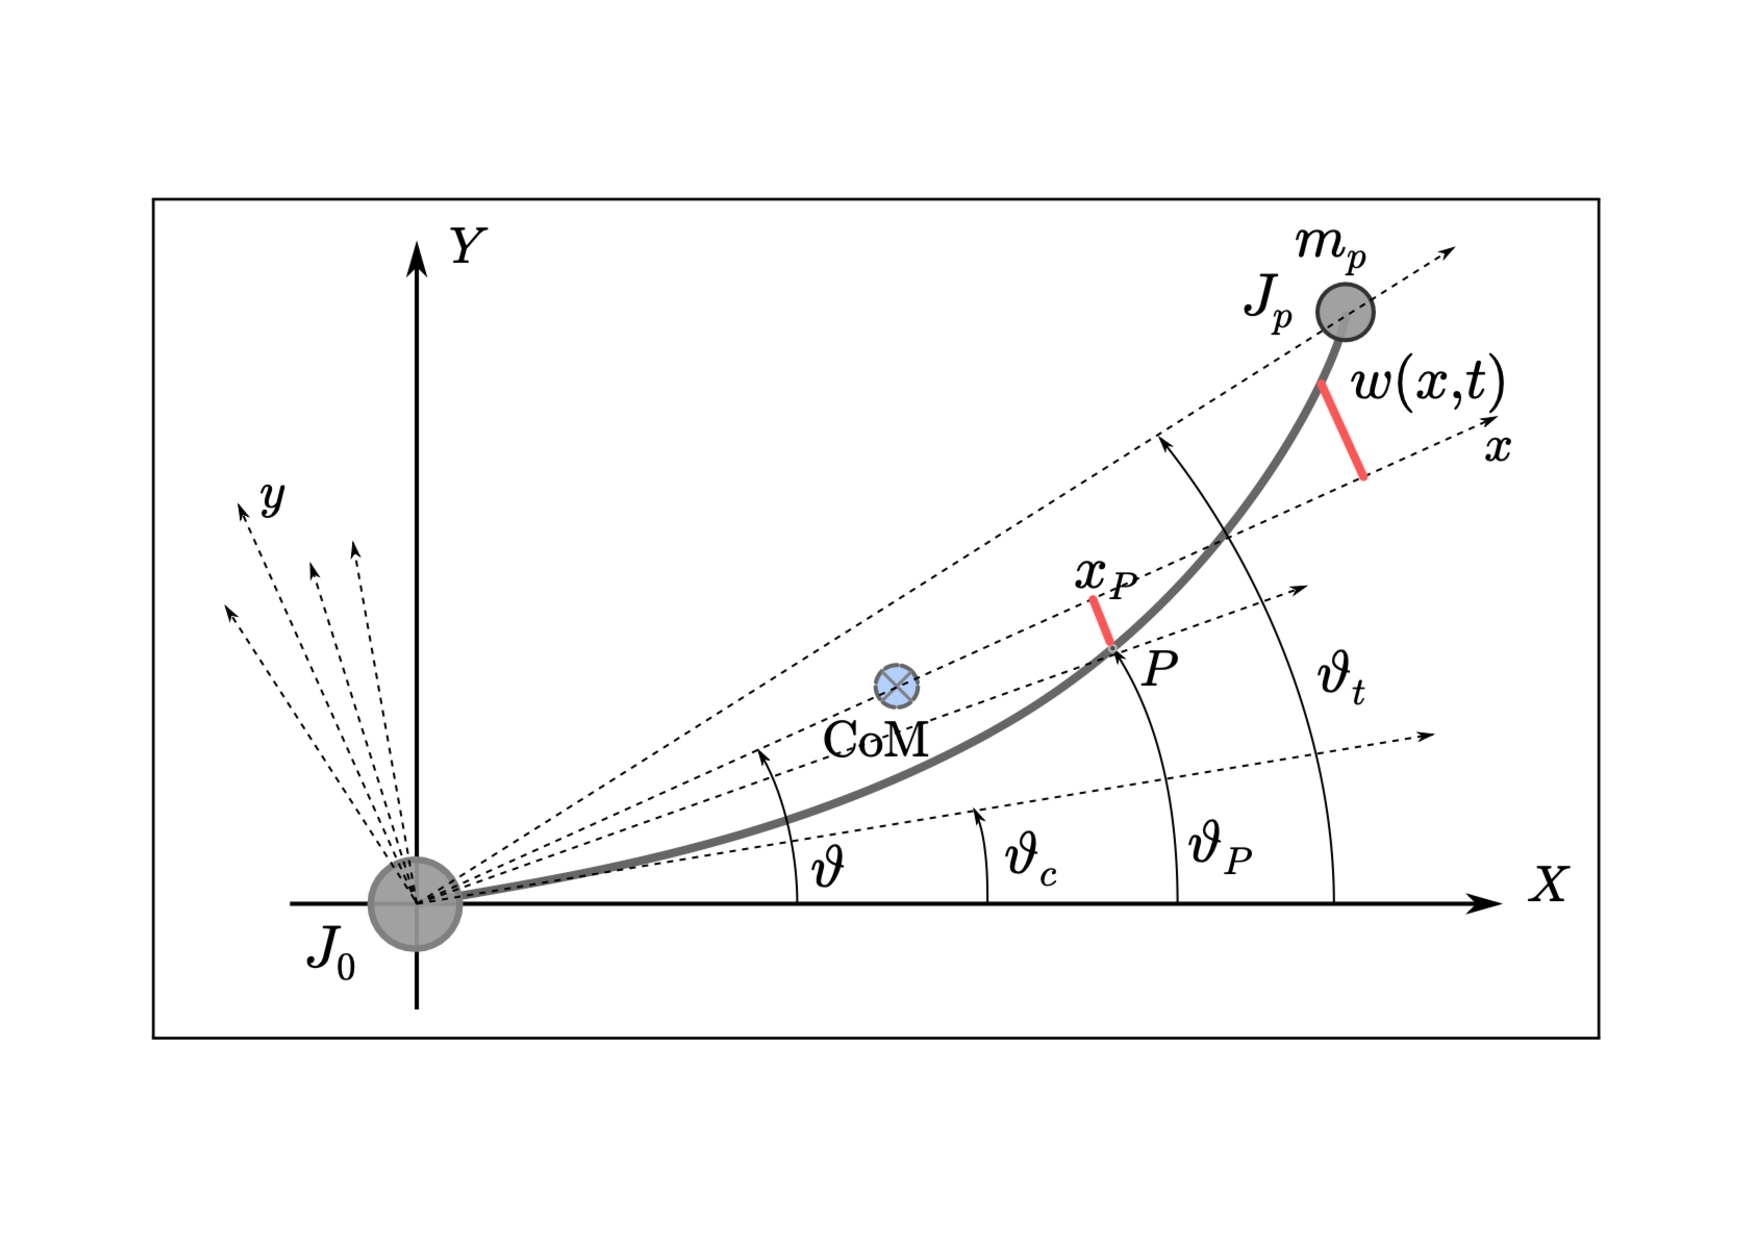
\includegraphics[width=0.5\textwidth]{Figures/fig01.pdf}}

\def\FigureTwo{\centering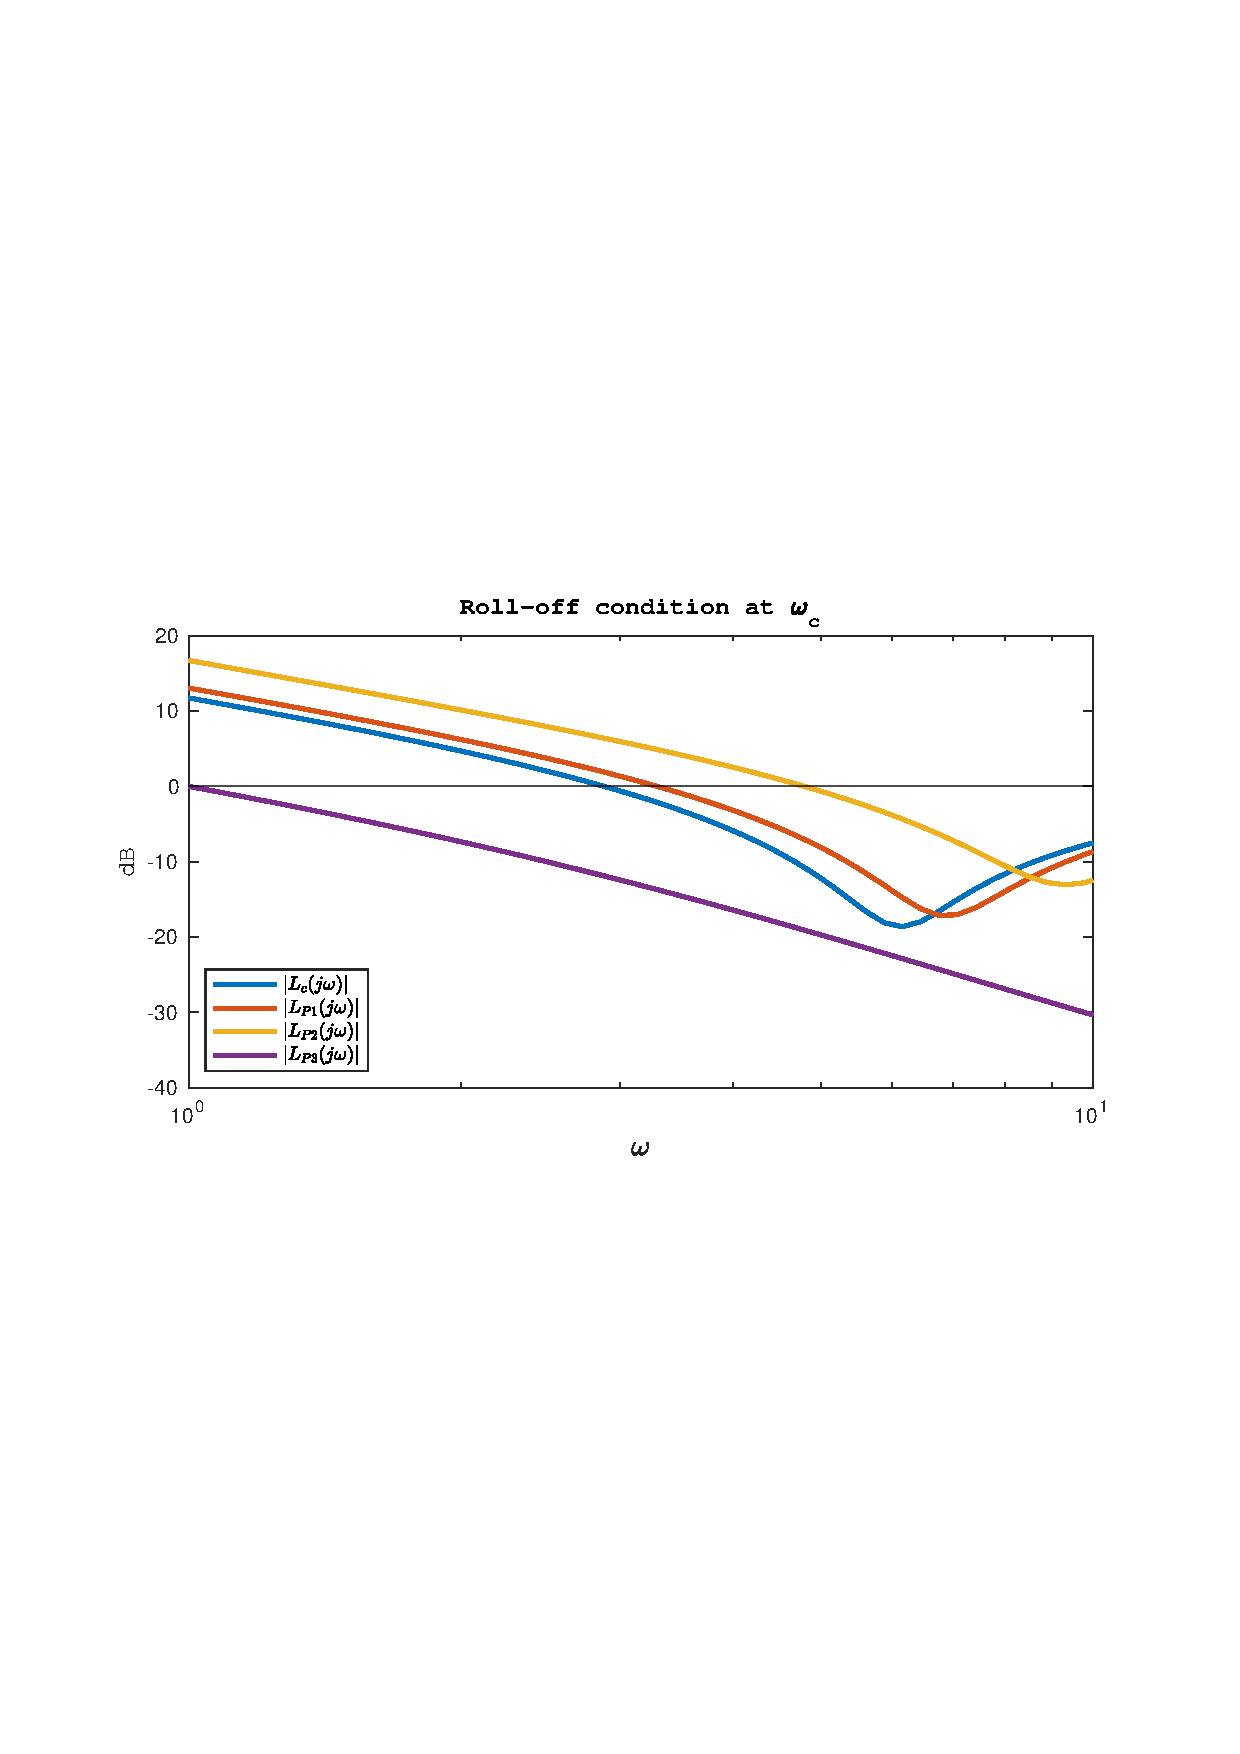
\includegraphics[width=0.7\textwidth]{Figures/fig02.pdf}}

\def\FigureThree{\centering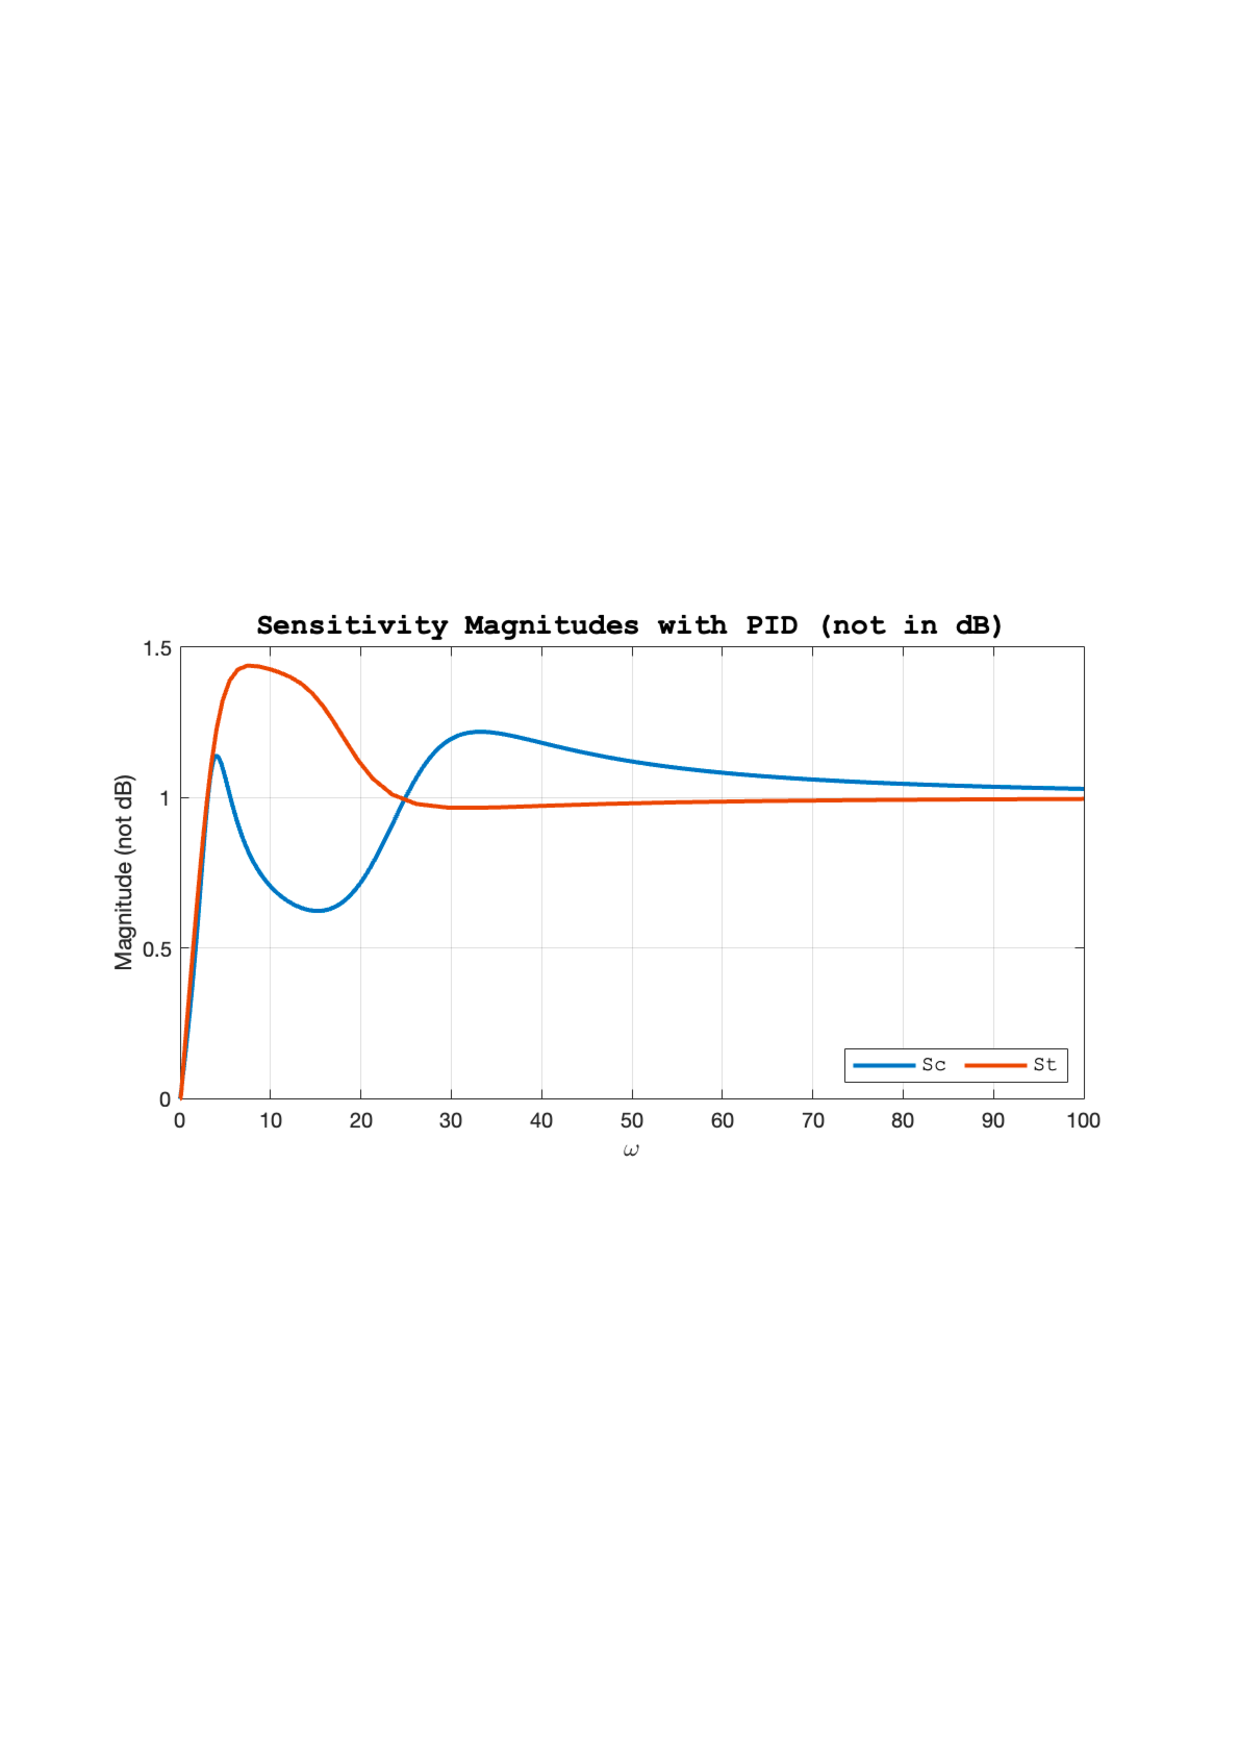
\includegraphics[width=0.7\textwidth]{Figures/fig03.pdf}}

\def\FigureFour{\centering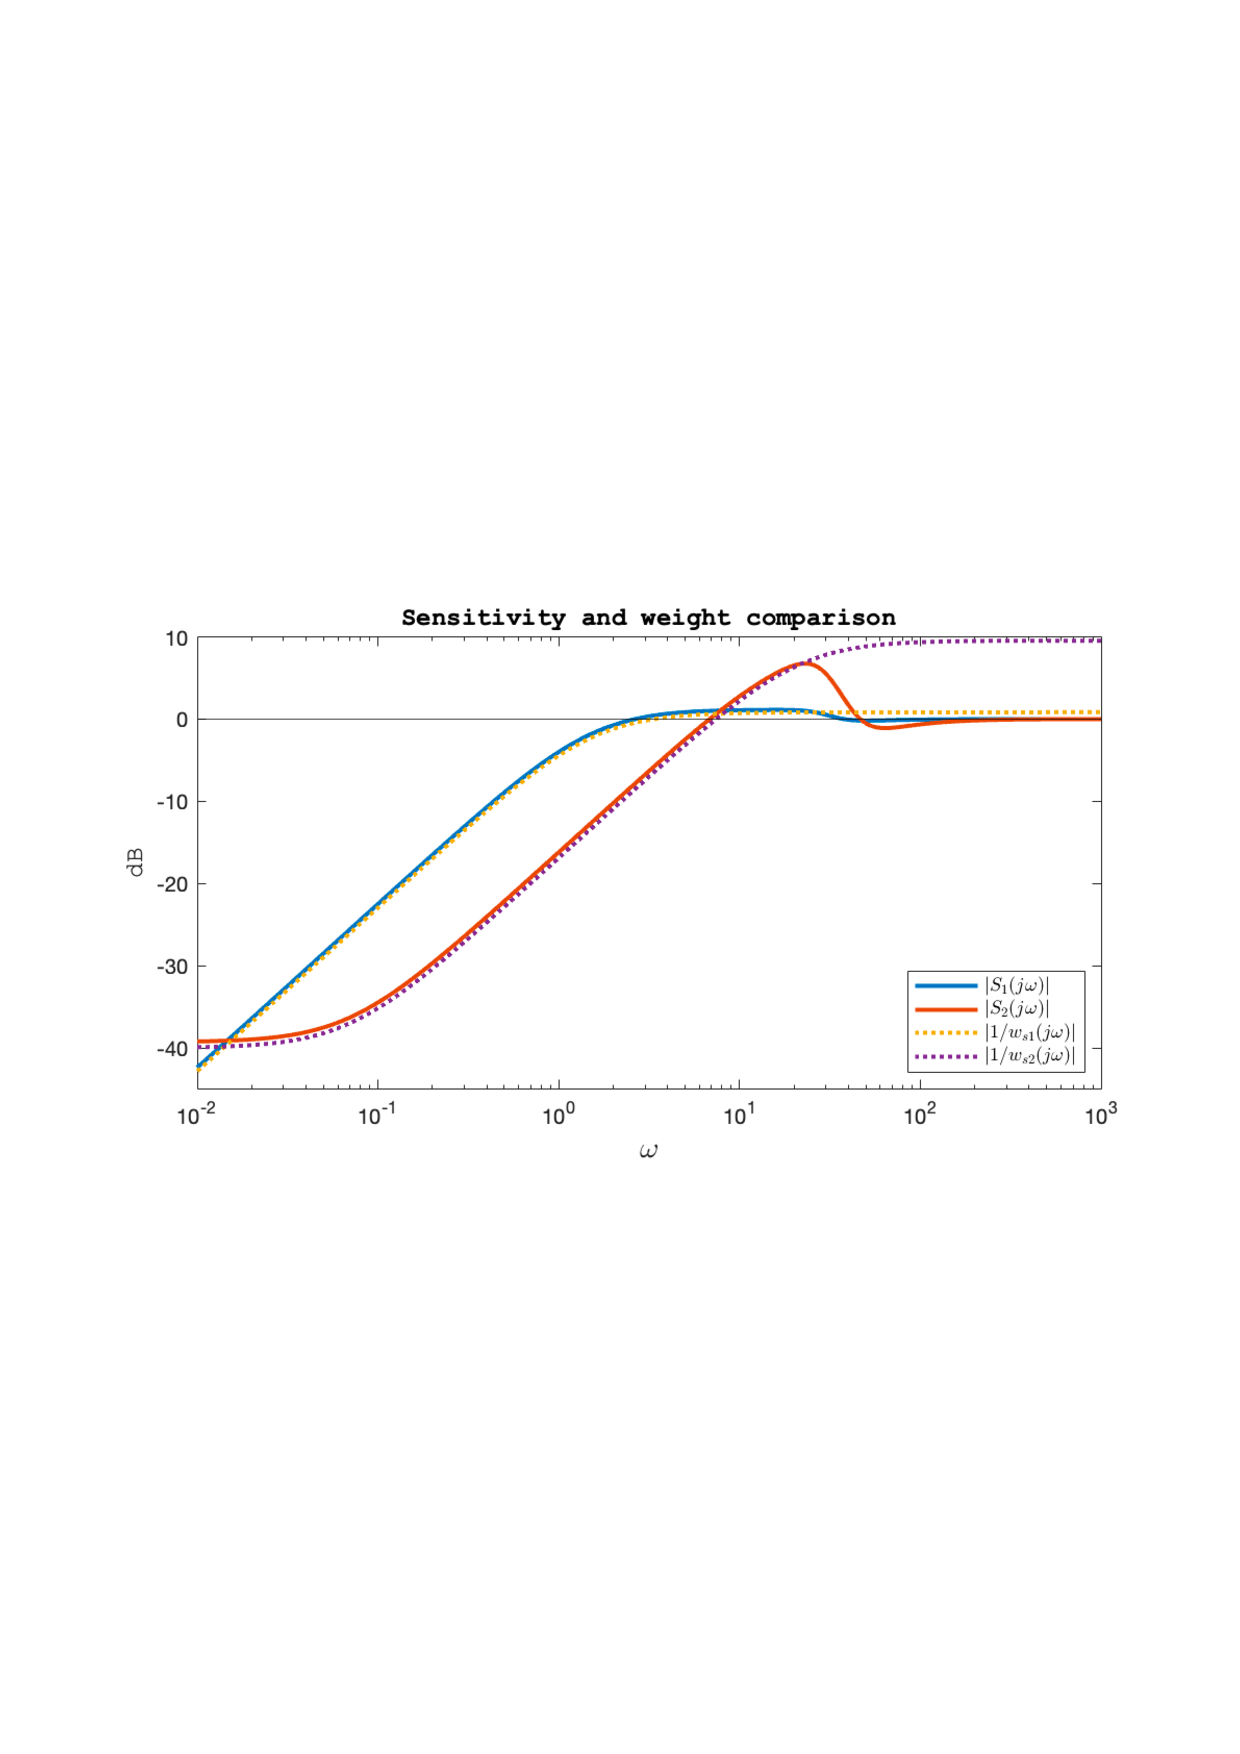
\includegraphics[width=0.6\textwidth]{Figures/fig04.pdf}}

\def\FigureFive{\centering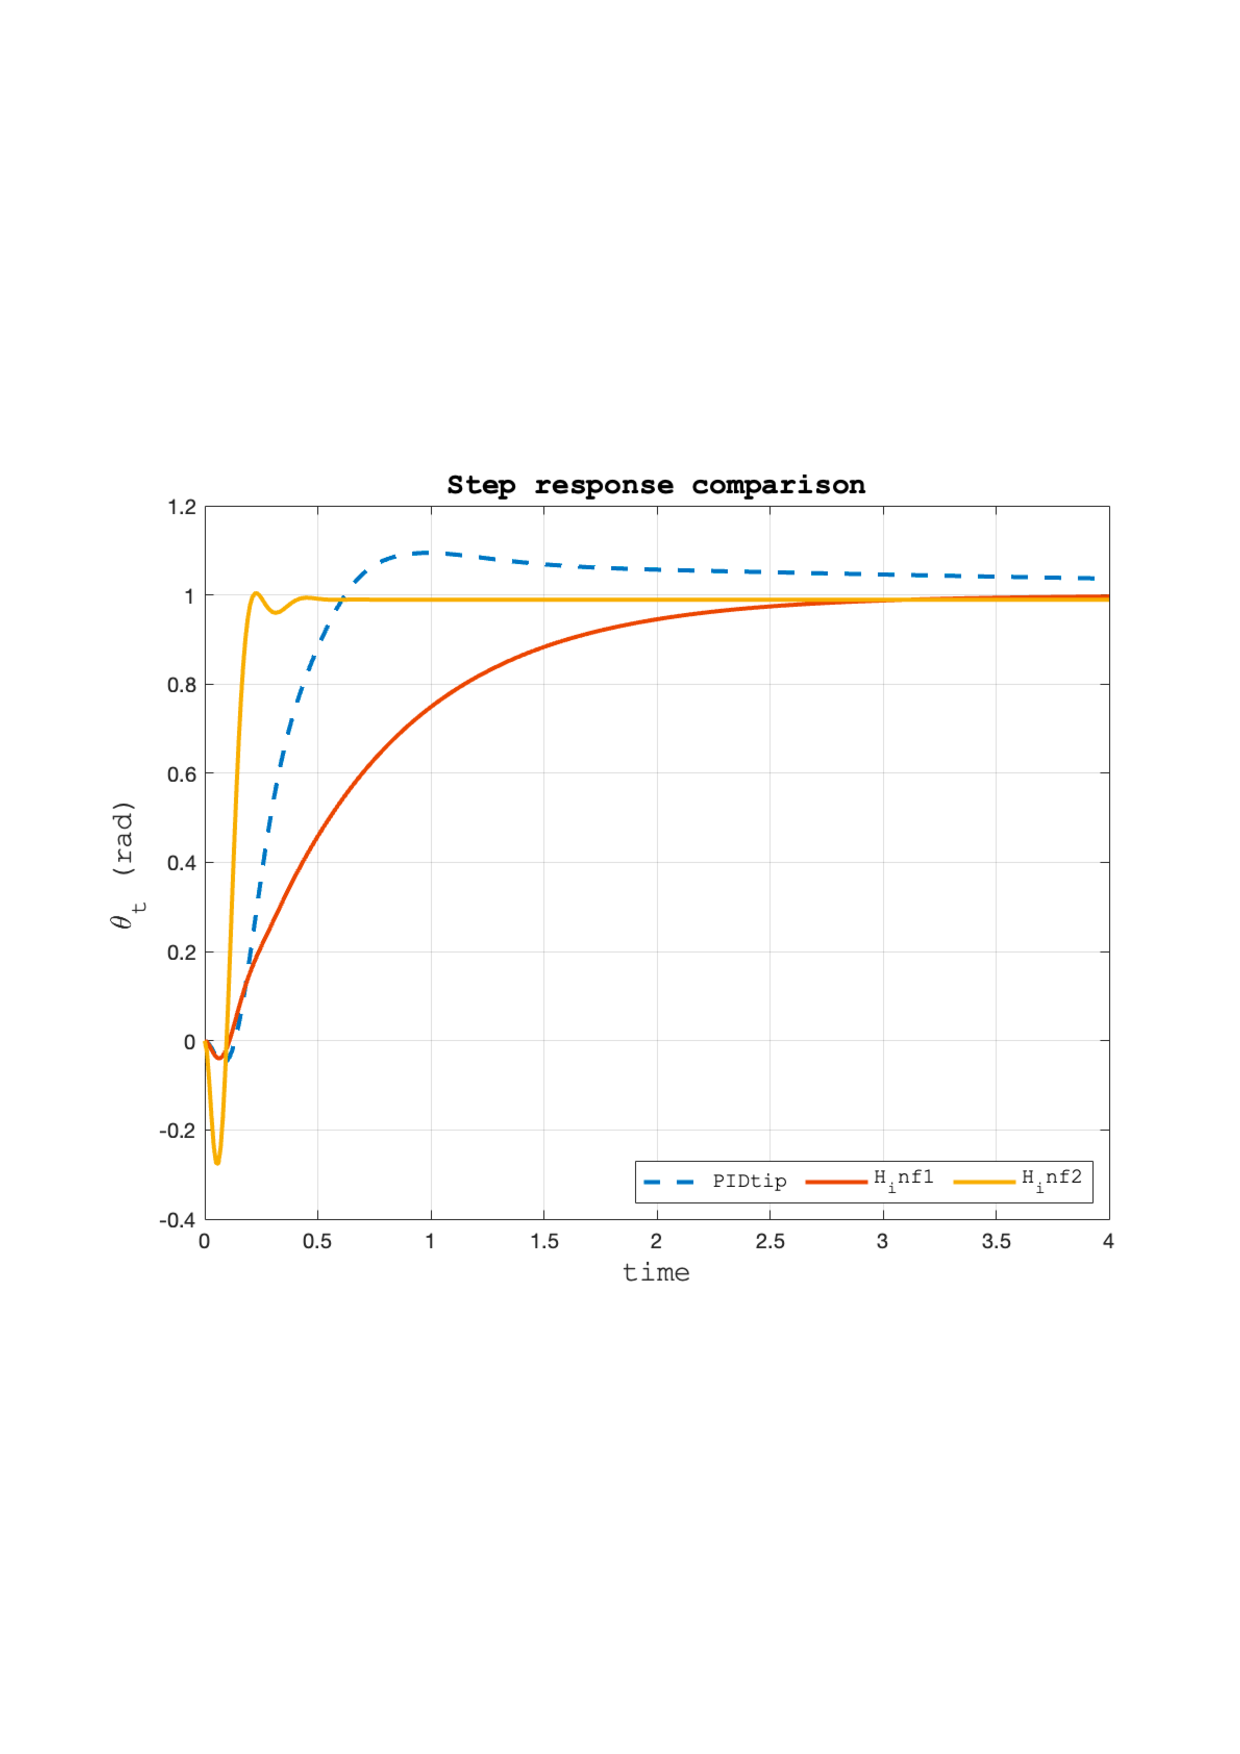
\includegraphics[width=0.8\textwidth]{Figures/fig05.pdf}}

\def\FigureSeven{\centering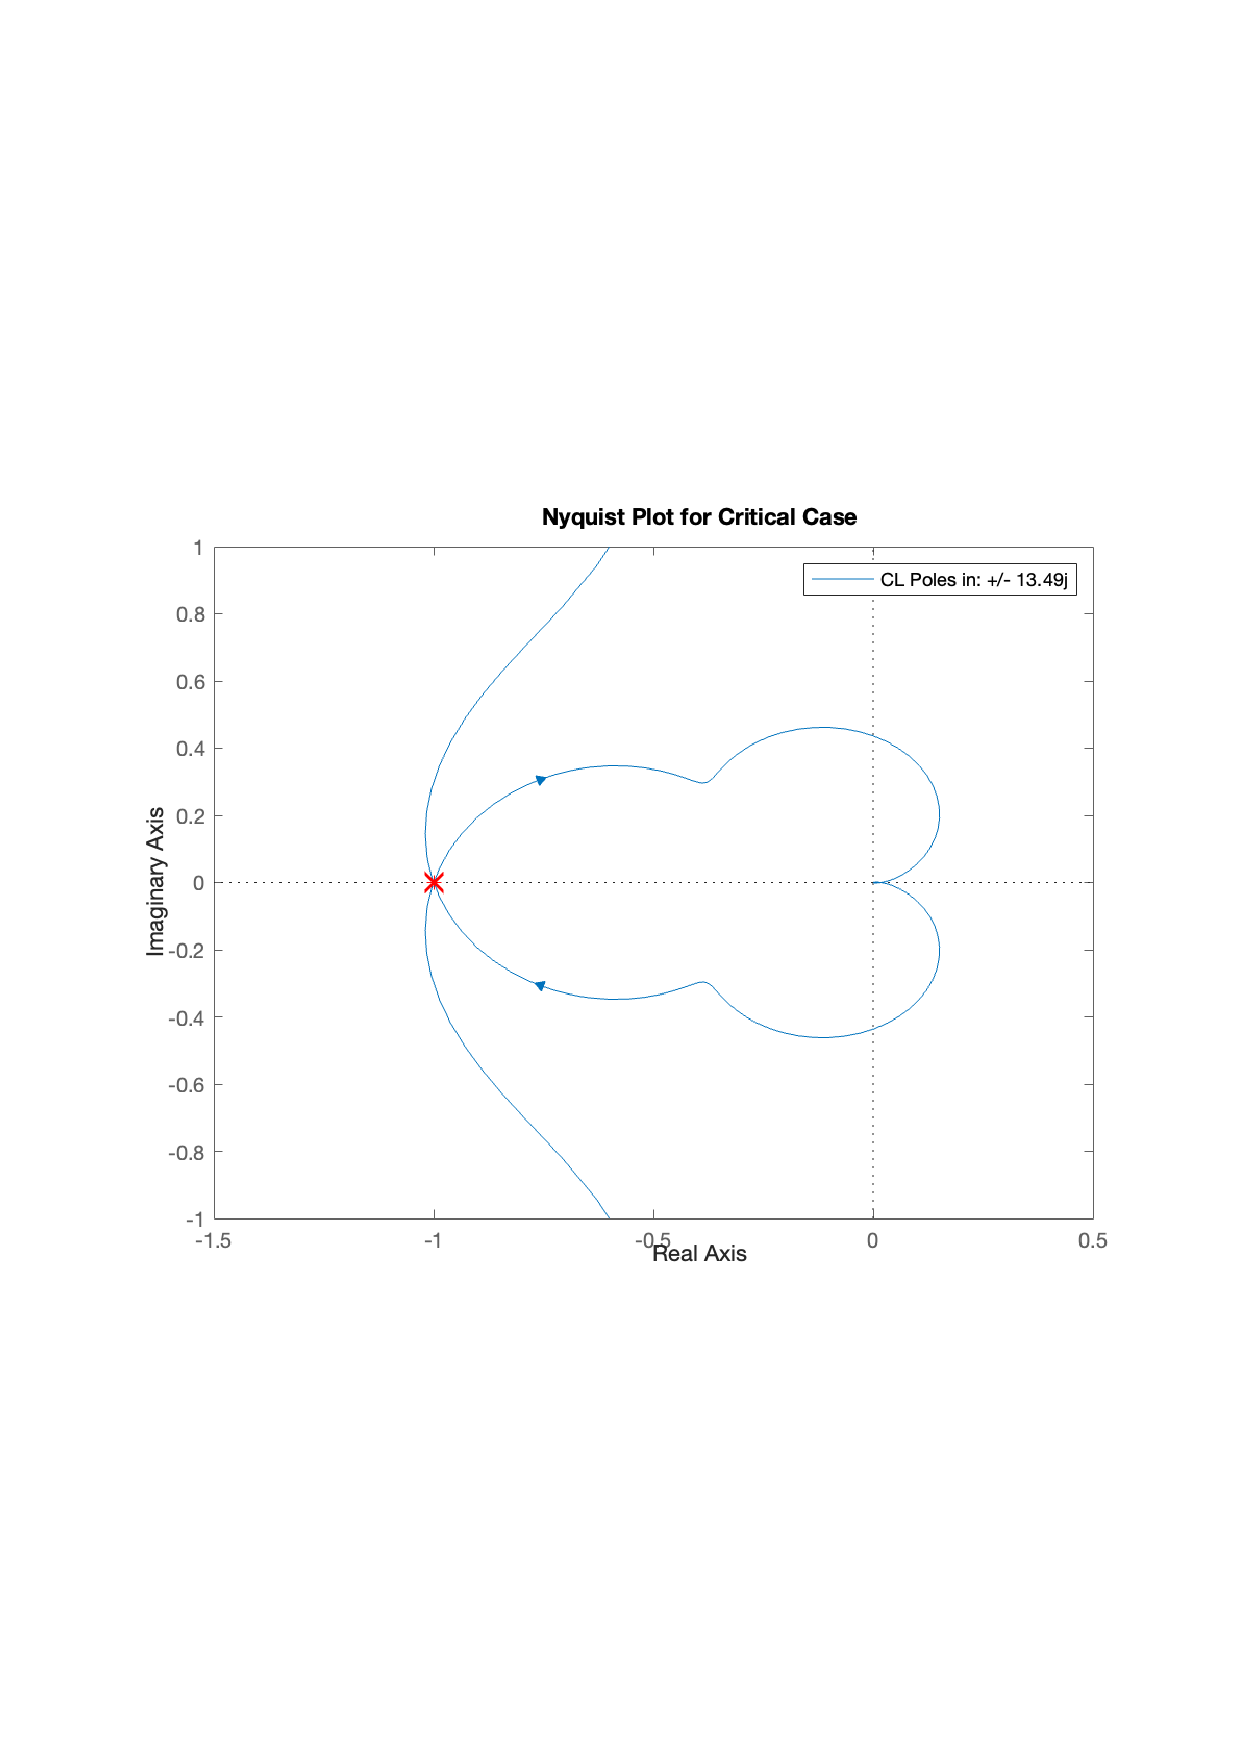
\includegraphics[width=0.8\textwidth]{Figures/fig07.pdf}}

\def\FigureEight{\centering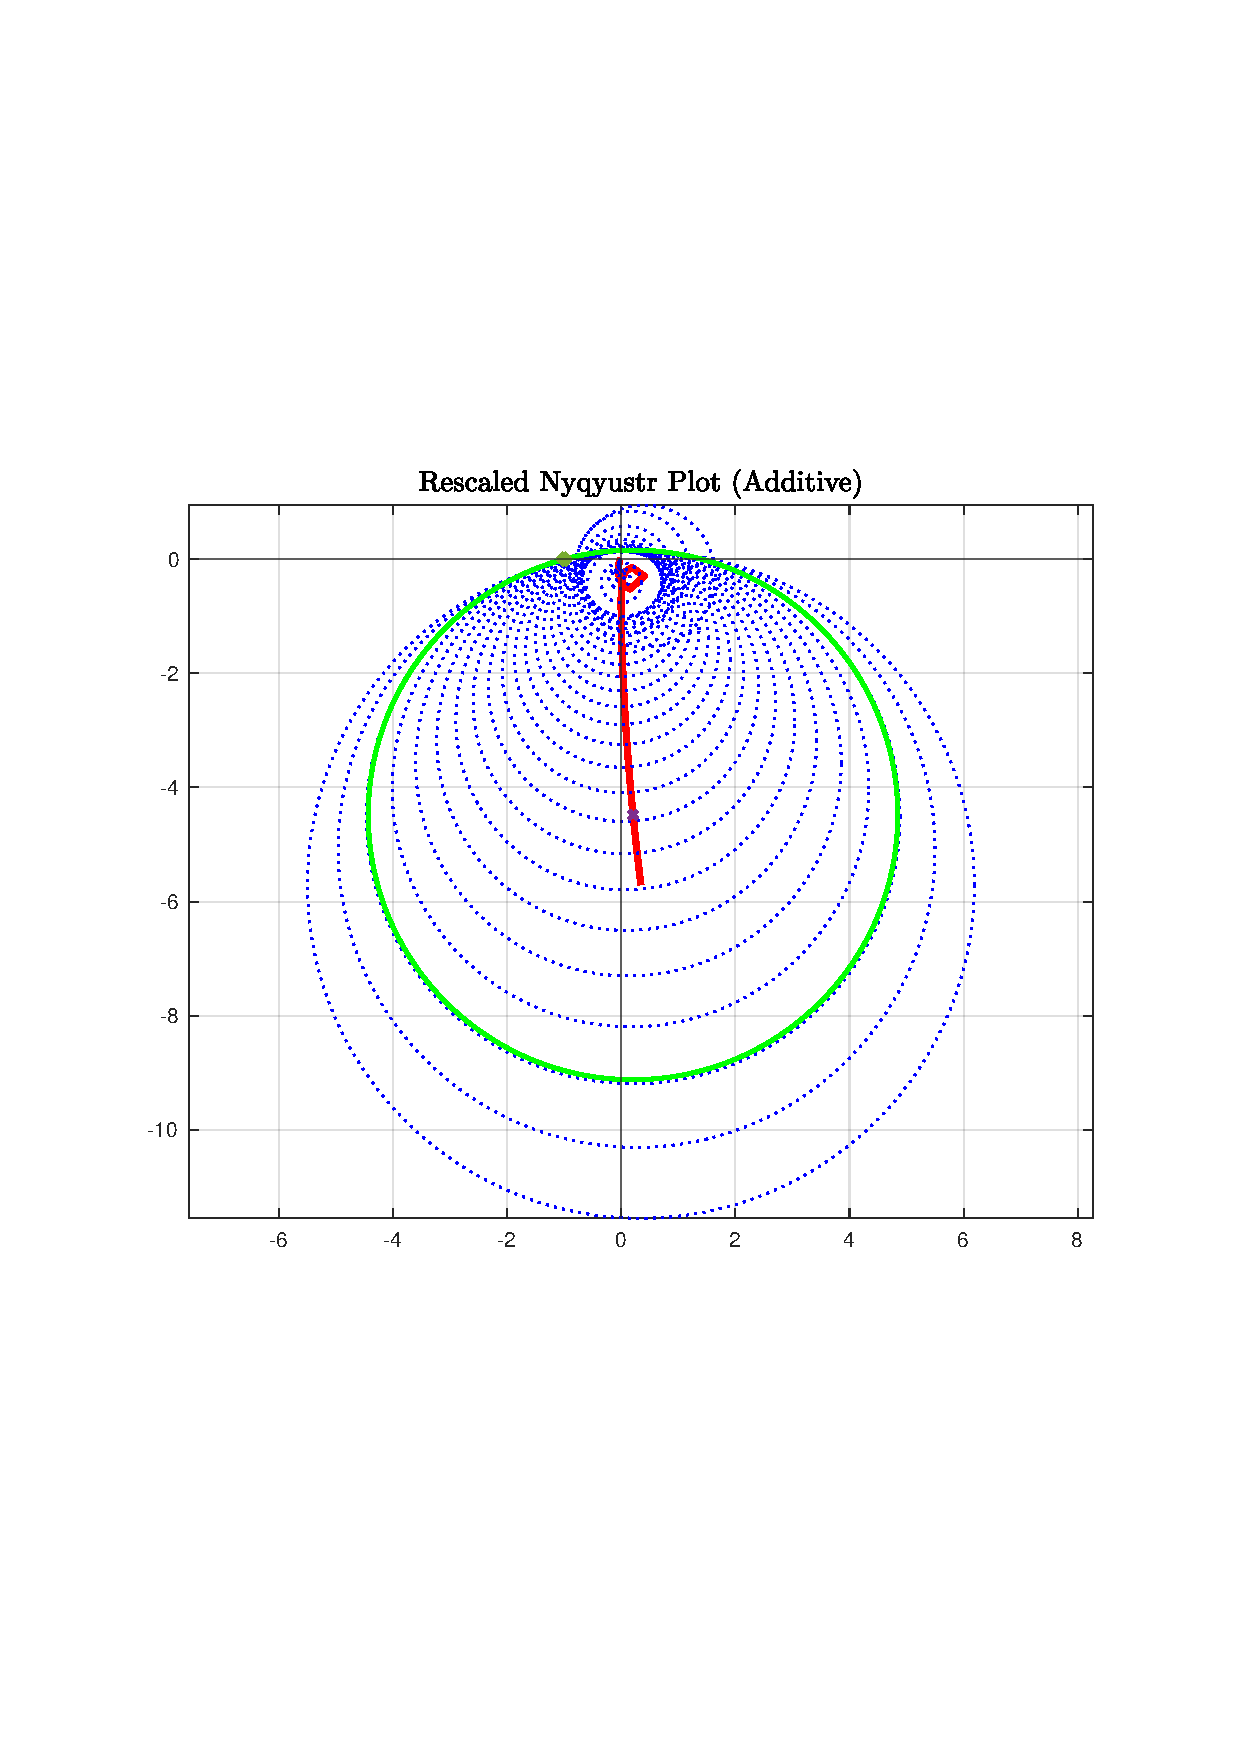
\includegraphics[width=0.8\textwidth]{Figures/fig08.pdf}}

\def\FigureNine{\centering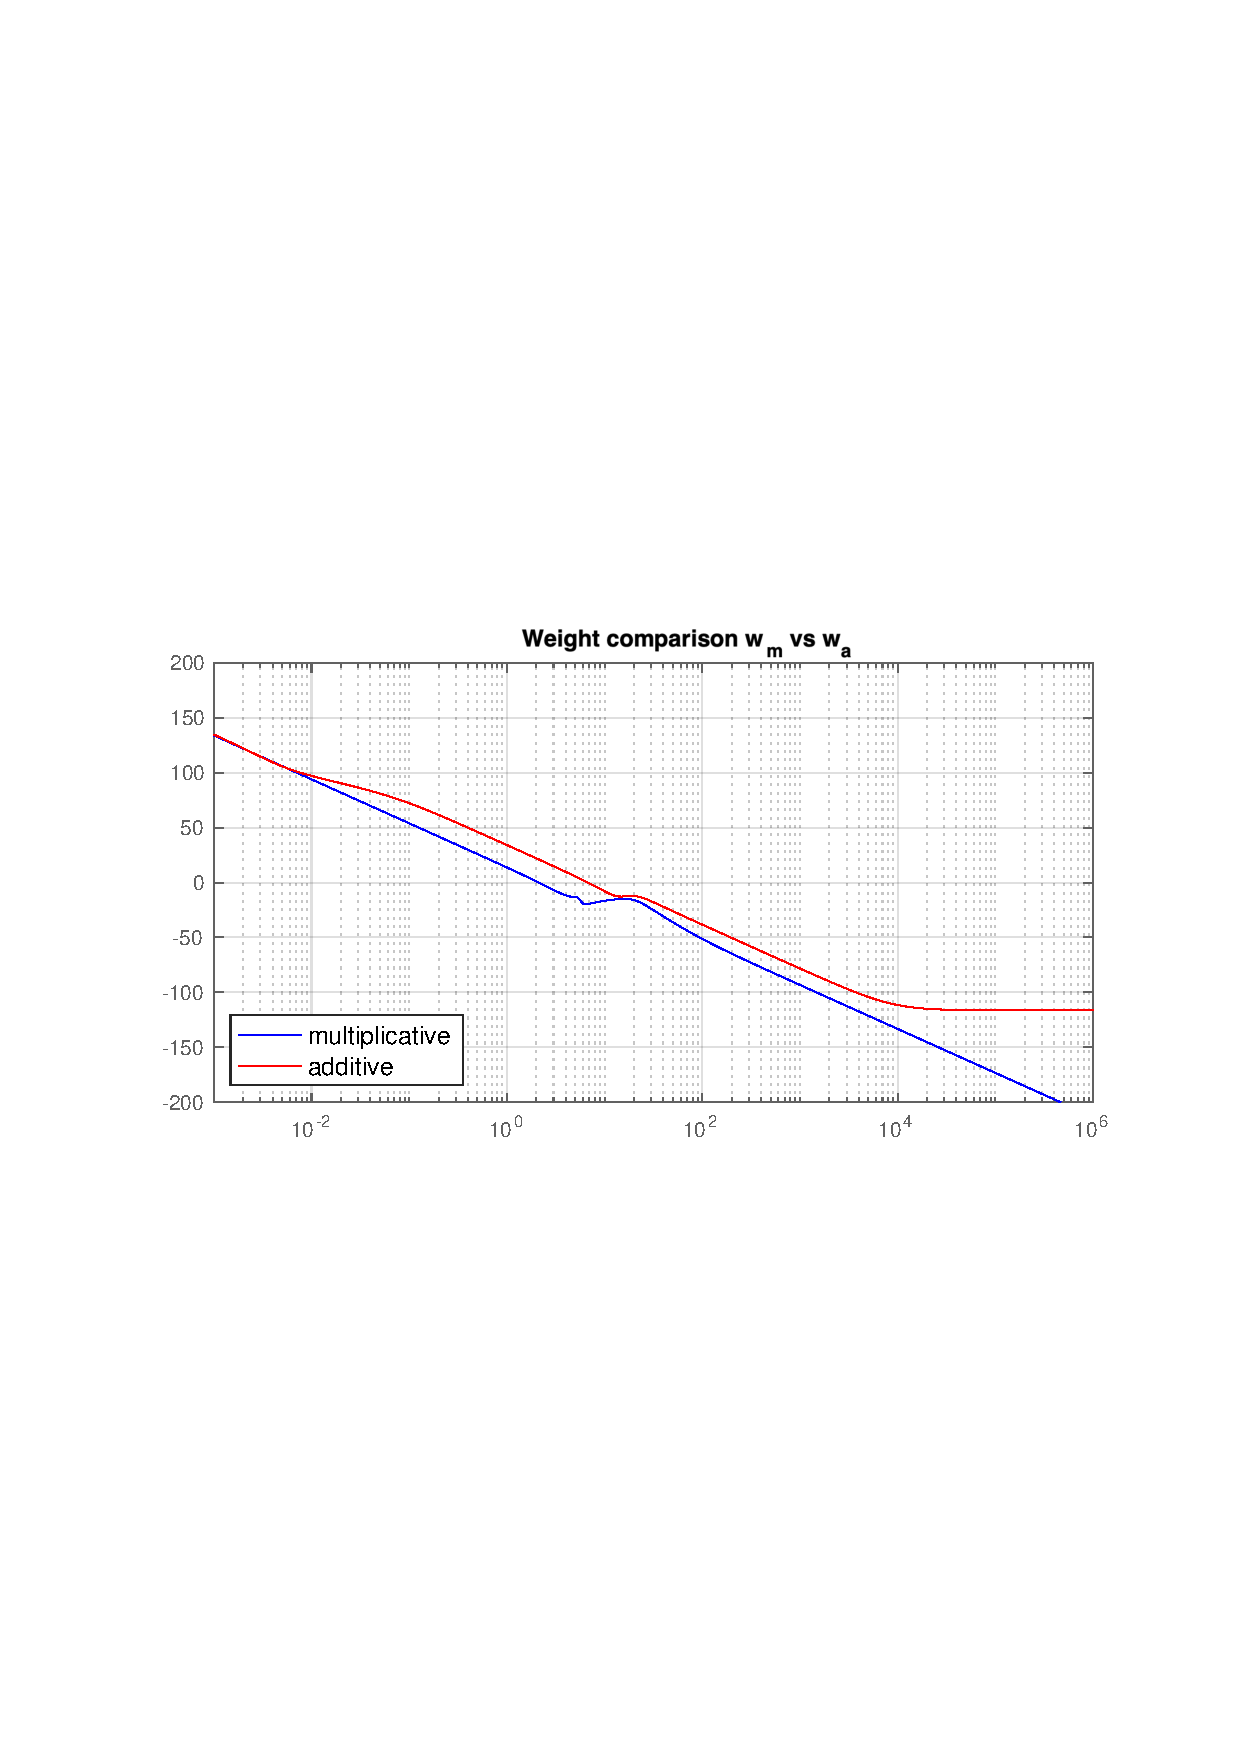
\includegraphics[width=0.8\textwidth]{Figures/fig09.pdf}}

\def\FigureTen{\centering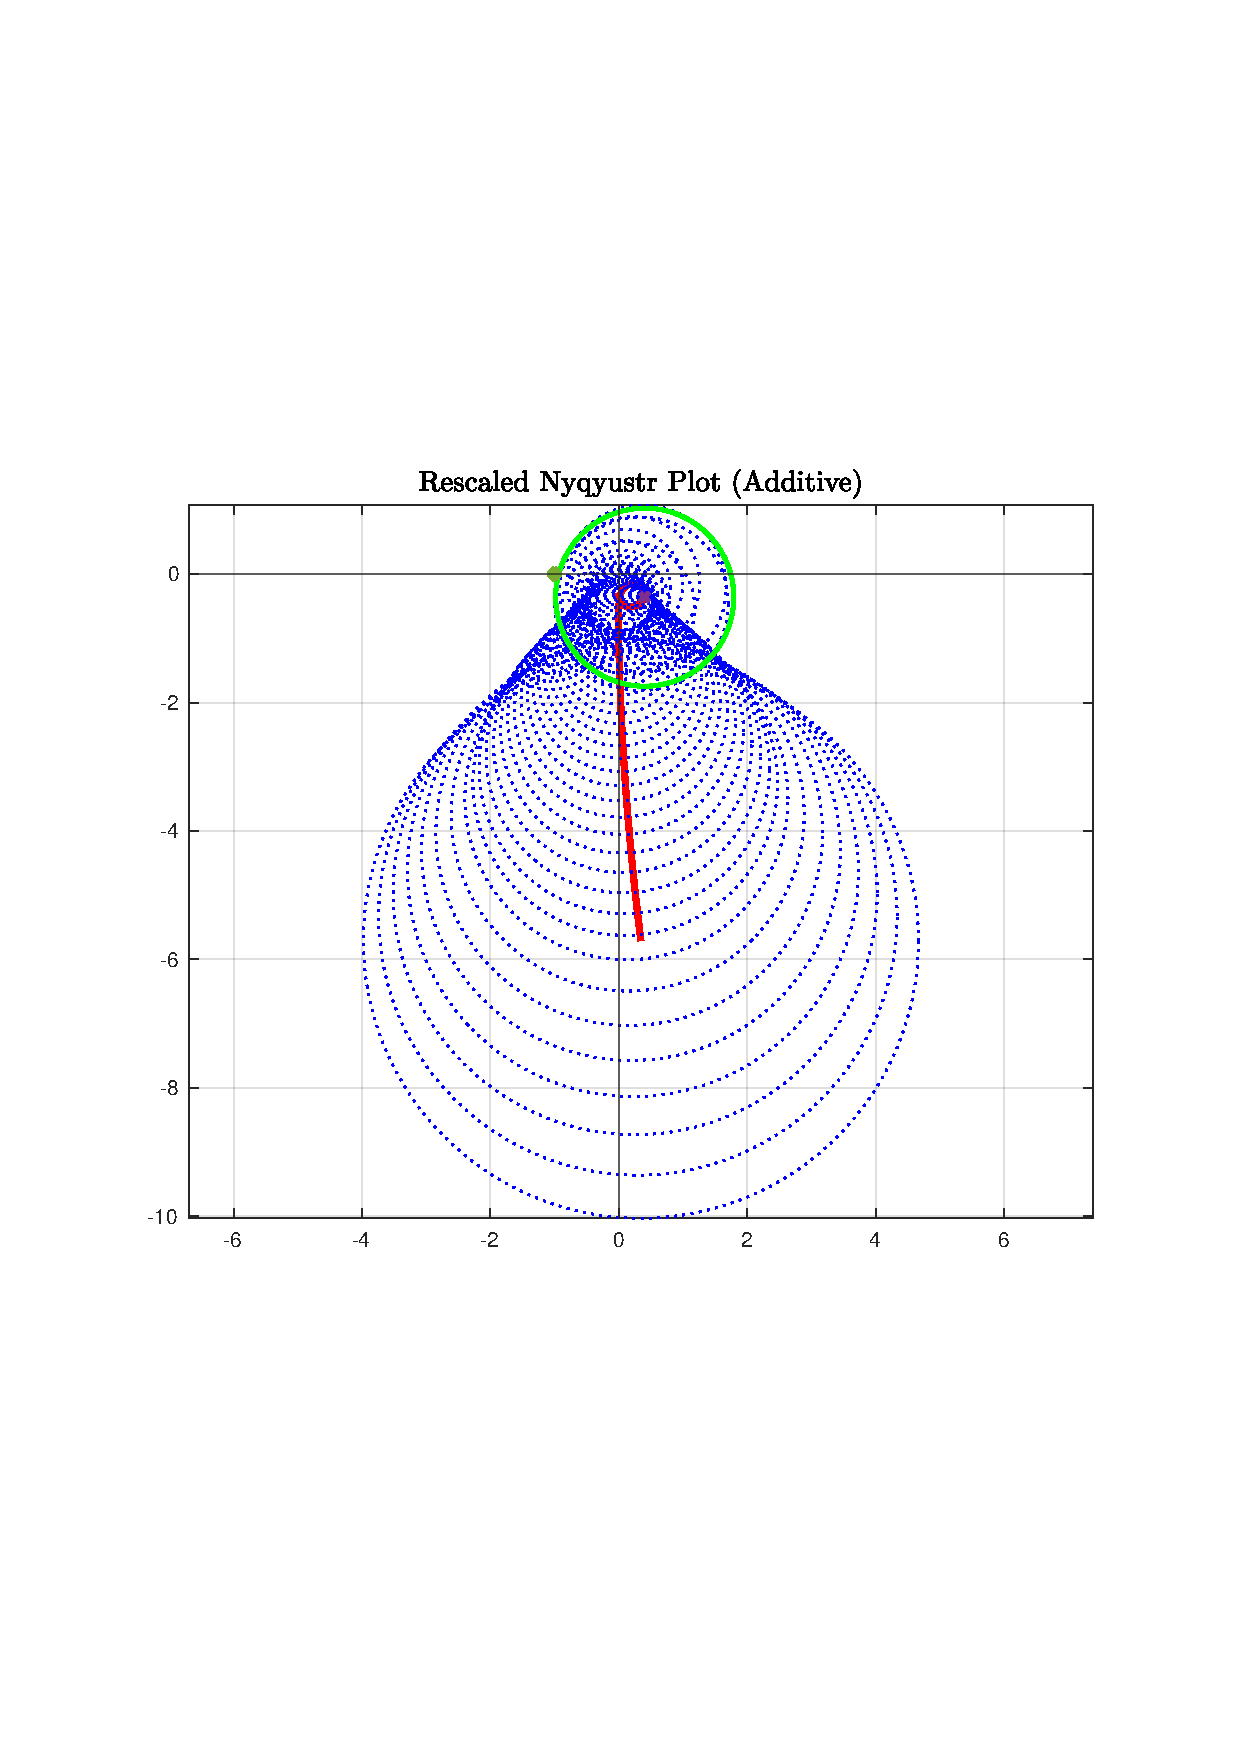
\includegraphics[width=0.6\textwidth]{Figures/fig10.pdf}}

\def\FigureEleven{\centering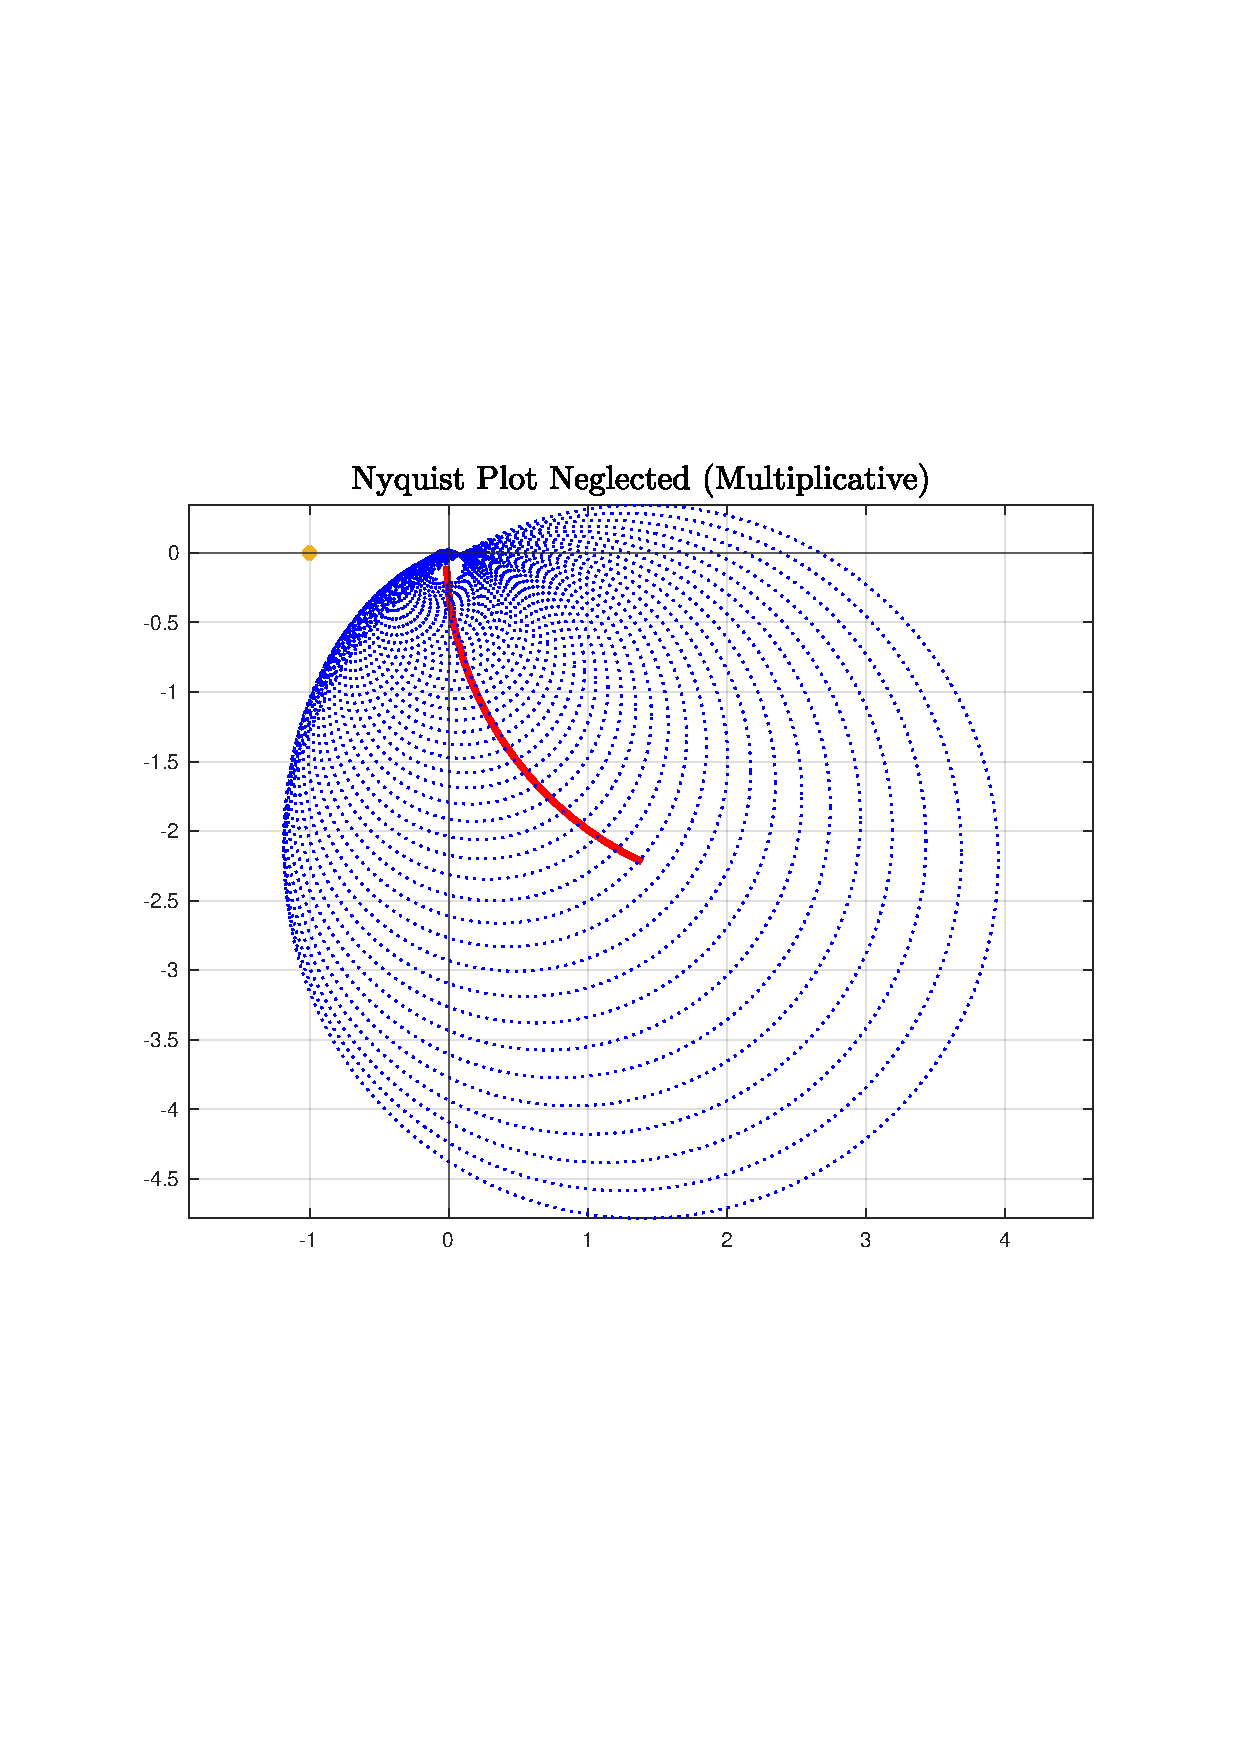
\includegraphics[width=0.5\textwidth]{Figures/fig11.pdf}}

\def\FigureTwelve{\centering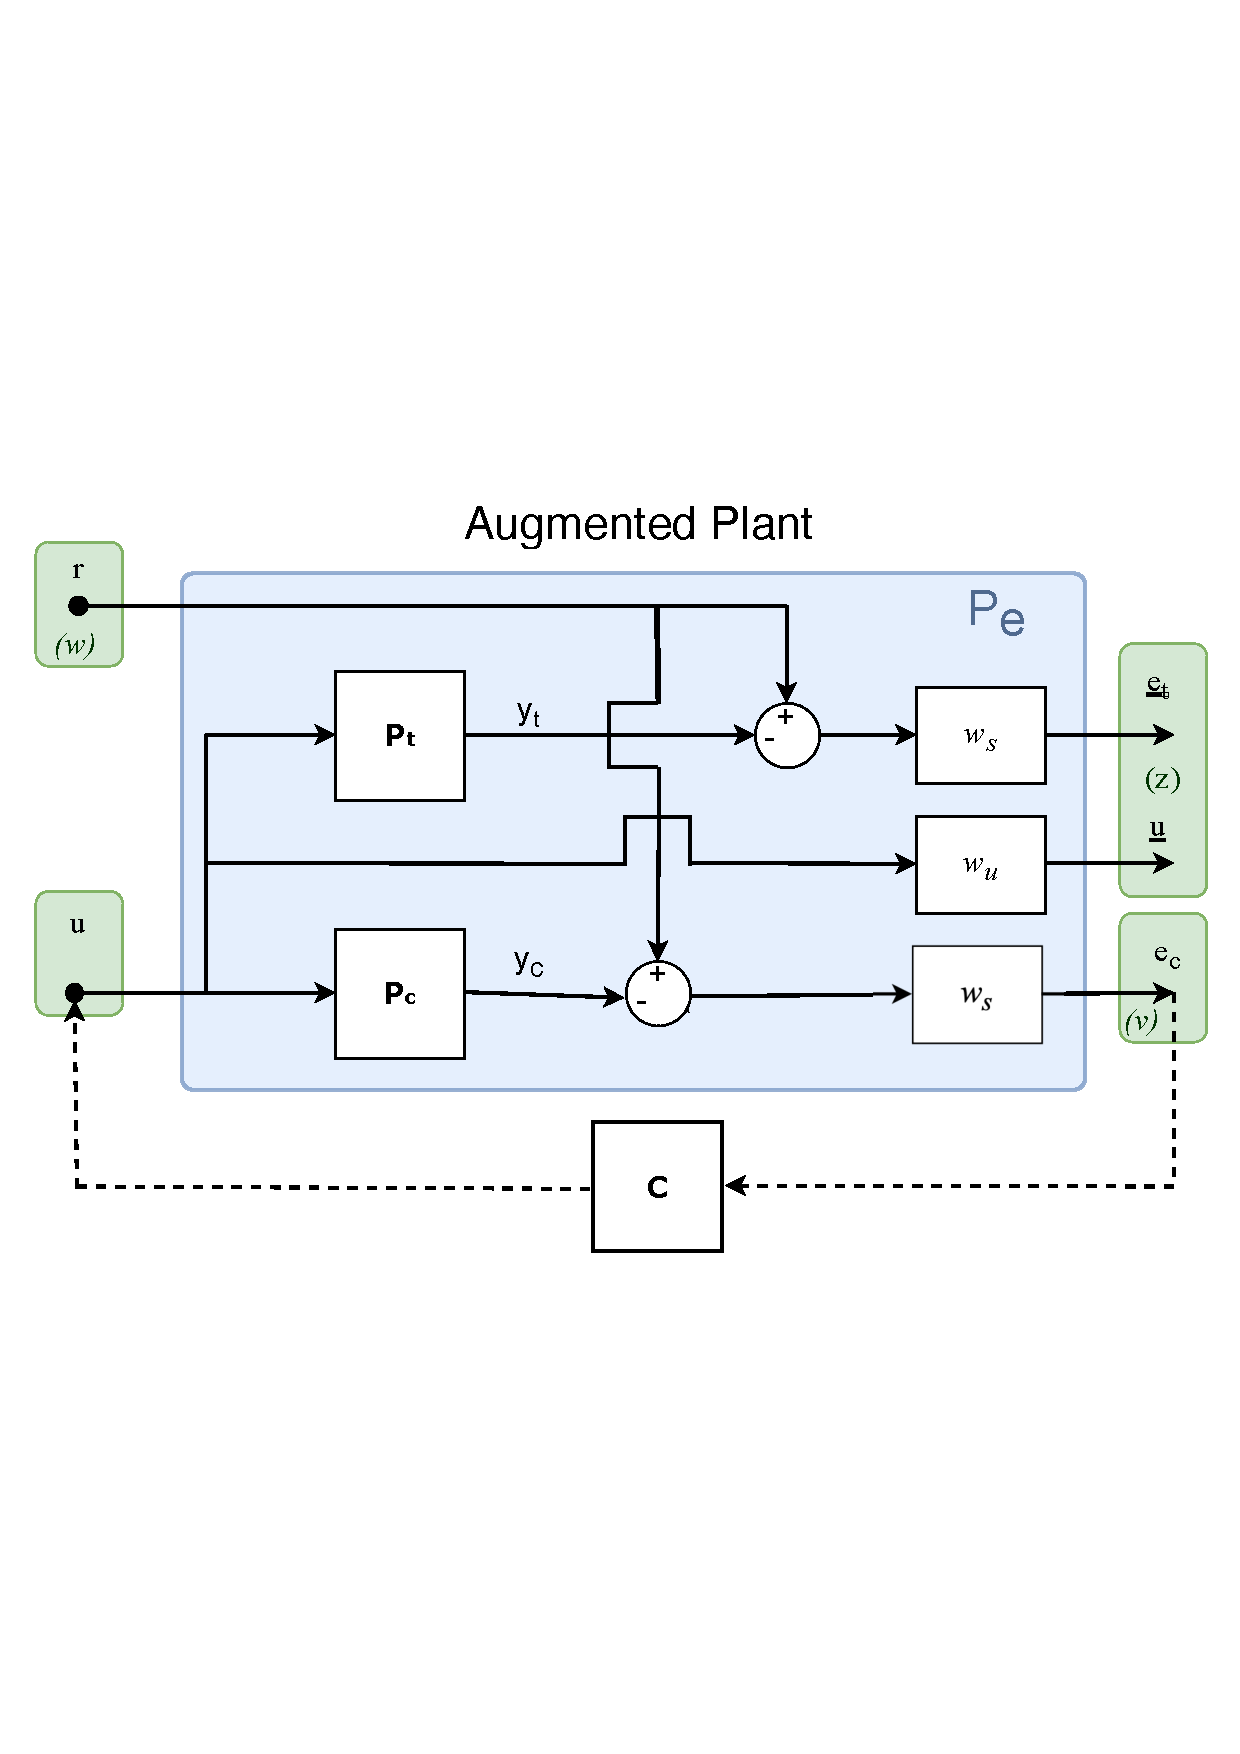
\includegraphics[width=0.75\textwidth]{Figures/fig12.pdf}}


\title{Multivariable Feedback Control \\ Homework 02}
\author{Matteo Scuderi\\ matricola 1937090}
\date{}

\begin{document}

\maketitle

\section{Problem 1: Limitations of Non Minimum Phase systems}

In this first problem I consider a flexible link of length $L$, actuated at the base, which can rotate on a plane, with respect to a fixed reference frame. The goal is to study how the input-output dynamics changes depending on the output chosen, and the limitations that arise from some particular choices. I assume that I'm asked to track a desired angular position $p\theta_{des}$, which for the moment will be assumed constant.\\
To highlight such limitations, I'll use a 1-DoF $H_\infty$ based controller.\\

\begin{figure}[h!]
    \FigureOne
    \caption{Single flexible link model}
    \label{fig:fig01}
\end{figure}

\subsection{Model description and analysis}
\label{sec:ModelDescription}
Without going in too much detail, under some assumptions, the infinite dimensional non-linear system can be simplified into a finite dimensional, linear one.\\
The dimensionality of the state space representation will be directly proportional to the number of modes considered in the approximation. At first, let's limit the analysis to the case $n_{modes} = 1$.\\\\
We can therefore consider, for the generic point $P$, the associated angle $\theta_P$. The associated Plant transfer function is:
\begin{equation}
        P_{\theta_P}(s) =\frac{1}{J} \frac{(1+J\Phi'(0)\Phi(x_P)/x_P) s^2 + 2\zeta_1\omega_1 s + \omega_1^2}
        {s^2 (s^2 + 2\zeta_1\omega_1 s + \omega_1^2)}
\label{eq:Model}
\end{equation}
\begin{itemize}
\item \textbf{J} $:=$ Total Inertia of the beam (beam + Tip)
\item \textbf{$\zeta_1$} $:=$ Damping ($\zeta_1 \in [0,1)$ )
\item \textbf{$\omega_1$} $:=$ Eigenfrequency of the first mode
\item   \textbf{$\Phi_1$} $:=$ Spatial shape of the deformed arm associated to the first mode 
\end{itemize}

\subsubsection*{Remark: Plant Transfer function}
We immediately notice that the any plant $P_{\theta_P}(s)$   has \textbf{relative degree r=2}. \\The system has two poles in zero and two stable poles (since $(\zeta_1, \omega_1) \geq 0$, the roots of the binomial term will have negative real part in presence of damping).\\
In the very special case in which $J\Phi'(0)\Phi(x_P)/x_P = 0$, the transfer function simplifies into a double integrator with gain $K = 1/J$.
\\\\More interestingly, the structure of the zeros of the plant only depends on the quantity $J\Phi'(0)\Phi(x_P)/x_P$. For having minimum phase system, we need to have $\Phi'(0)\Phi(x_P)/x_P > -1/J$. This always holds true when the the spacial deformation at the generic point $X_p$ has the same sign as $\Phi'(0)$. However, the more the point approaches the tip, the more negative (if $\Phi'(0) > 0$) the second value will be. Therefore, especially if the inertia J grows, there exists a set of points $X_{NMP} := [\overline{x_P}, L]$ for which $J < -\Phi'(0)\Phi(x_P)/x_P$, hence \textbf{the system considered is not minimum phase}.


\subsection{Models' construction}
With the choice of parameters reported in the Matlab files,we have no load at the tip and subsequently rather low inertia J.\\
We choose three kind of outputs to try to capture the essence of the problem in question:\\
\begin{itemize}
\item\textbf{Joint Angle $\theta_c$}: angle at the beam base
\item\textbf{Tip angle $\theta_t$}: angle at the tip approximated by $\theta_c + \sum_{i=1}^{n_e}\frac{\Phi_i(L)}{L}$
\item\textbf{$x_P$ angle $\theta_P$}: angle at a fixed point $x_P$ approximated by $\vartheta_c + \sum_{i=1}^{n_e}\frac{\Phi_i(L)}{L}$
\label{sec:Modelconstruction}
\end{itemize}
We place three points strategically at $x_{P_i} = \{\frac{L}{4},\frac{L}{2},\frac{3L}{4}\}$ and compute the transfer functions.
\subsubsection*{Remark: Non minimum phase Plant}
As previously discussed, the minimum-phase property depends on the sign and value of $\Phi'(0)\Phi(x_P)/x_P$.\\
For the points $x_P = L/4, L/2$, the quantity $\Phi(x_P)/x_P$ is positive, and therefore the inequality $\Phi'(0)\Phi(x_P)/x_P > -1/J$ is trivially satisfied.\\
For the point $x_P = 3L/4$, we have a negative spacial deformation, but the inequality is still satisfied, hence the system is still minimum phase.
\\Finally, for the plant relative to the \textbf{tip angle}, we have $\Phi'(0)\Phi(x_P)/x_P < -1/J$ and $P_t(s)$ is indeed \textbf{non minimum phase}.\\\\Notice that having low inertia implies that the inequality is "harder to break", but just adding some mass at the tip could change significantly the plants, making the set $X_{NMP}$ larger.

\subsection{Limitations' Analysis}
As first approach, to understand the limitations that arise from the non-minimum phase property, we'll use some "dummy" PIDF controllers, so we can close the loop and study the sensitivities. We'll restrict the comparison to the $P_t(s)$ and $P_c(s)$ plants (relative to the tip and base angle respectively).
\subsubsection{Open loop limitations: roll-off condition}
Using the "dummy" PID controllers, we can verify that the roll-off condition holds true for each minimum phase open loop system.
Plotting the Bode magnitudes, we can observe (Fig.~\ref{fig:fig02}) that none of the slopes exceeds the bound of the roll-off condition: they're all below 40 dB/dec. This same condition will hold true for any controller we might design, therefore it's useless to try to shape the loop function to have a larger slope around the crossover frequency.
\begin{figure}[h!]
    \FigureTwo
    \caption{Loop functions satisfying roll-off condition}
    \label{fig:fig02}
\end{figure}


\subsubsection{Sensitivities and Sensitivities' Integrals}
I used two "baseline" controllers $C_{PIDc},C_{PIDt}$, each one tuned appositely on the respective plant, with a design focus on reference tracking (the tuning is made with Matlab's $pidtune(\dots)$).
The respective sensitivities are reported in the graph below (Fig.~\ref{fig:fig02}) and we call $S_t(j\omega)$ the Sensitivity relative to the tip angle and $S_c(j\omega)$ the one relative to the base angle: 
\begin{figure}[h!]
    \FigureThree
    \caption{Sensitivities of $P_t$ and $P_c$ (not in dB)}
    \label{fig:fig03}
\end{figure}
Since we have both systems having relative degree equal 2 and no poles in the right half plane, we can calculate the Bode Sensitivity Integral for $P_c$ (minimum phase) and the Poisson Integral for $P_t$ (n.m.p.). Calling $z \approx 16.45$ the right half plane zero, we have, as expected:
\\\\
\begin{itemize}
    \item $\int_{0}^{\infty} \ln \left| S_c(j\omega) \right| \, d\omega = 0$
    \item $\int_{0}^{\infty} \ln \left| S_t(j\omega) \right|\frac{2z}{z^2+\omega^2} \, d\omega = 0$
\end{itemize}

\subsubsection{Minimum Phase system Analysis}
The first result, for the minimum phase plant, testifies the fact that we cannot make $|S_c(j\omega)|<1$ for any $\omega$, therefore it's impossible to reject disturbances at all frequencies. Moreover, if we consider this integral in terms of a sum of "positive" and "negative" area, we know that they need to cancel out. Therefore we might be subject to large sensitivity peaks if we try to push the crossover frequency (i.e. increase the "negative area").
\\
To make things more clear, we can think of the integral as a sum of three parts: the "positive area" (which might contain the peak), the "negative area" and the \textbf{Sensitivity Tail}. \\
\\ The tail contribution to the integral however is approximately null, therefore our goal is to find a certain frequency $\omega_{tail}$ up until which we consider the integral contribution as relevant. On the other hand, the infinite integral from $\omega_{tail}$ to infinity will be approximated to zero. 
\\\\
Hence, we must fix an $\epsilon$ small enough, such that $|L_c(j\omega)| < 1\ \forall \omega < \omega_{tail}$. Once we've found such frequency, we have that the following inequality holds true:
\begin{itemize}
    \item$\int_{\omega_{tail}}^{\infty} \ln \left| S_c(j\omega) \right| \, d\omega < \omega_{tail} \ln(\frac{1}{1-\epsilon})$
\end{itemize}
Choosing an $\epsilon$ small enough, we can make the approximation of the tail to zero more and more accurate, but at the same time $\omega_{tail}$ will grow larger and larger.
\\\\
Most importantly, this implies that the "sensitivity area" must cancel out in the frequency range prior to $\omega_{tail}$, since after that the contribution is close to null. Pushing the crossover frequency closer to $\omega_{tail}$ will cause a peak just before the tail frequency.

\subsubsection*{Remark: Matlab implementation and results}
To find the $\omega_{tail}$, I've used the function $freqresp(L_c,100:1:200)$, which evaluates the Loop transfer function (assuming $L = P_cK$) over the frequency range of 100:200 (since we're looking for an upper bound, we don't care about extreme precision).   
\\Then we fix our $\epsilon = 0.01$ and look for the frequency starting form which $|L_c(j\omega)| < 1$, which will be approximately our $\omega_{tail}$. Finally, we check that the integral defined above is indeed bounded by that constant, which is exactly the case.
\\
\subsubsection{Non minimum phase analysis}
The second result $\int_{0}^{\infty} \ln \left| S_t(j\omega) \right|\frac{2z}{z^2+\omega^2} \, d\omega = 0$ is "bad news" in terms of design, since it indicates that we're subject to the second waterbed effect. In fact, we have that the Bode Sensitivity integral from 0 to $z_{RHP}$ is close to zero. This implies that "most of the positive area" is spread before the right half zero frequency. Pushing bandwidth will only cause higher and higher peaks, the more we approach $z_{RHP}$. 

\subsection{Design Limitations}
Let's focus now, for the design, on the non minimum phase plant. For the waterbed effect, we know that increasing "negative area" in the sensitivity, for instance pushing bandwidth, will cause an higher peak ("positive area") and thus worse performance, with more oscillatory behavior in the transient.
\\Therefore, we need to be careful assigning the weight $w_S$ for the sensitivity, while performing $H_\infty$ control.
\\\\Keeping in mind that we need to have $\left| w_S(z) \right| < 1$ , we can make several choices.\\
To highlight the waterbed effect, let's pick two controllers
$C_{t1}$ and $C_{t2}$. The first one is designed on a "compromise" paradigm: lower bandwidth ($B3 \approx 1.4$) to reduce "negative area" and $M = 1.1$. The second one is designed with a "greedy" approach: high bandwidth ($B3 \approx 8$) and $M = 2$ to "mitigate negative area".\\
The Control Sensitivities are bounded (by choice) by two constant weights $w_{S_u}$ equal to 0.1 and 0.02 respectively, since higher bandwidth demands an higher bound for the control sensitivity. Resulting sensitivities are shown below: 
\begin{figure}[h!]
    \FigureFour
    \caption{Sensitivities comparison with the two controllers: waterbed effect}
    \label{fig:fig04}
\end{figure}
It's no surprise to see (Fig.~\ref{fig:fig04}): how the step response (to the complementary sensitivity) is shaped. The PID response is also reported as reference. \\Overall performance has surely been improved, with much reduced tracking error. The "greedy" $H_\infty$ controller has more oscillations, but also a very short rise time due to high bandwidth. However, it's not feasible in real life due to extremely high control effort requirements.  
\begin{figure}[h!]
    \FigureFive
    \caption{Step response comparison with the $H_\infty$ controllers}
    \label{fig:fig05}
\end{figure}
\section{Extension: Multiple modes}
Let's now consider multiple modes (in particular, we pick $n_e = 3$) and see how the situation changes.
The model's matrices are now: 
\begin{equation*}
    M = \begin{bmatrix}
    J & 0  & 0  & 0\\
    0 & 1 & 0  & 0\\
 0 & 0 & 1  & 0\\
 0 & 0 & 0  & 1 \quad
 \end{bmatrix}
D = \begin{bmatrix}
0 & 0 & 0 & 0\\ 
0 & 2 \zeta_1 \omega_1 &0 & 0\\
0 & 0 &  2 \zeta_2 \omega_2 & 0\\
0 & 0 & 0 &  2 \zeta_3\omega_3
\end{bmatrix}
K = \begin{bmatrix}
0 & 0 & 0 & 0\\
0 & \omega_1^2 & 0 & 0\\
0 & 0 &  \omega_2^2 & 0\\
0 & 0 &  0 & \omega_3^2\cr 
\end{bmatrix} \quad
B_p = \begin{bmatrix}
1 \cr \Phi'_1(0) \\ \Phi'_2(0)  \\
\Phi'_3(0)
\end{bmatrix}
\end{equation*}
We obviously notice and increase in dimensionality of our models. The system's transfer functions have now 8 poles ($n_p = 2(n_e + 1)$) and 6 zeros ($n_z = 2n_e$).\\
We also notice that the non-minimum-phase plant $P_t$ has now \textbf{three zeroes in the right half plane}, one real and two complex conjugates.
\\ \\ \\
We try to design our new controllers for the $P_t,\ P_c$ plants with the same exact sensitivity weights as per their single-mode counterparts. We end up with a slightly more oscillating behavior (due to the presence of more complex poles). This is mostly evident for the m.p. $P_c$, whose closed loop performance degrades significantly.
\\ \\
Surprisingly enough, the n.m.p. plant maintains almost the exact same performance with the new $H_\infty$ controller.\\ The presence of the two complex RHP zeros doesn't seem to compromise the performance.\\

\clearpage
\section{Problem 2: Robustness}
The second problem we want to study is robustness with respect to uncertainties in the model. Once again, let's limit the analysis to the $P_t(s)$ and $P_c(s)$, to compare minimum vs non minimum phase behavior, and use the $H_\infty$ controllers designed for Problem 1. 
\\ To do so, we'll explore different sources of uncertainty and different ways of modeling such uncertainty. In particular, we'll explore:
\begin{enumerate}
    \item \textbf{Structured (real) parametric uncertainty}
    \item \textbf{Unstructured (full complex) parametric uncertainty}
    \item \textbf{Unmodelled dynamics (from model approximations)}
    \item \textbf{Neglected dynamics}
\end{enumerate}
\subsection{Uncertain Model}
The biggest source of a uncertainty that can occur in a real world scenario, can surely be the \textbf{presence of a load at the tip} of the flexible robot's arm. In the model, such mass $M_t$ has so far been considered equal to zero. To be more consistent with real life applications, when studying robust stability, we're going to consider $M_t \in [0,0.5]Kg$. Even if this parameter doesn't appear directly in our model, its value affects directly all other parameters (think of inertia). Moreover, since the \textbf{damping coefficient} is by definition subject to errors and approximations, we consider also a 10\% error on the nominal value $\zeta_{nom}$.
\subsubsection{Uncertain Mass at Tip}
\textbf{We model the load at the tip as a sphere} or radius $R=0.1\ m$. \\The total inertia is hence $J_{tot} = J_{link}+M_tL^2 + J_{tip} = J_{link}+M_t(L^2+\frac{2}{5}R^2)$.
\\From now on, instead of considering the uncertainty on the Mass at the tip, we'll use the uncertainty of the other parameters \textbf{related to that mass}, such as inertia. All computations are made in the external file $EulerBeam\_Modeling1Mode\_Uncertain.m$.
\subsubsection{Range of the Model's Parameters}
Making all the computations, we end up with \textbf{6 uncertain parameters} (for computational issues, in the Matlab file the variable $\omega^2$ is considered as a sixth uncertain parameter):\\
\begin{itemize}
    \item $\zeta_{unc} \in [0.36, 0.44]$ 
    \item $J_{unc} \in [0.169,0.671]$
    \item $\Phi_{unc}'(0) \in [6.02,7.83]$
    \item $\Phi_{unc}(L) \in [-2.7,-0.471]$
    \item $\omega_{unc} \in [13.9,20.5]$
\end{itemize}
The first one is the damping coefficient, which has an uncertainty of 10\%. Everything else is related to the mass at the tip and varies in its own range.\\  
We generate such uncertain parameters with the $ureal()$ command. 
\subsection{Structured (real) parametric uncertainty}
The resulting uncertain plants, letting the \textbf{real parameters} vary in their range, with some sampling of course, have the following bode plots (Fig.~\ref{fig:fig06}):
\begin{figure}[h!]
    \centering
    \begin{subfigure}[b]{0.45\textwidth}
        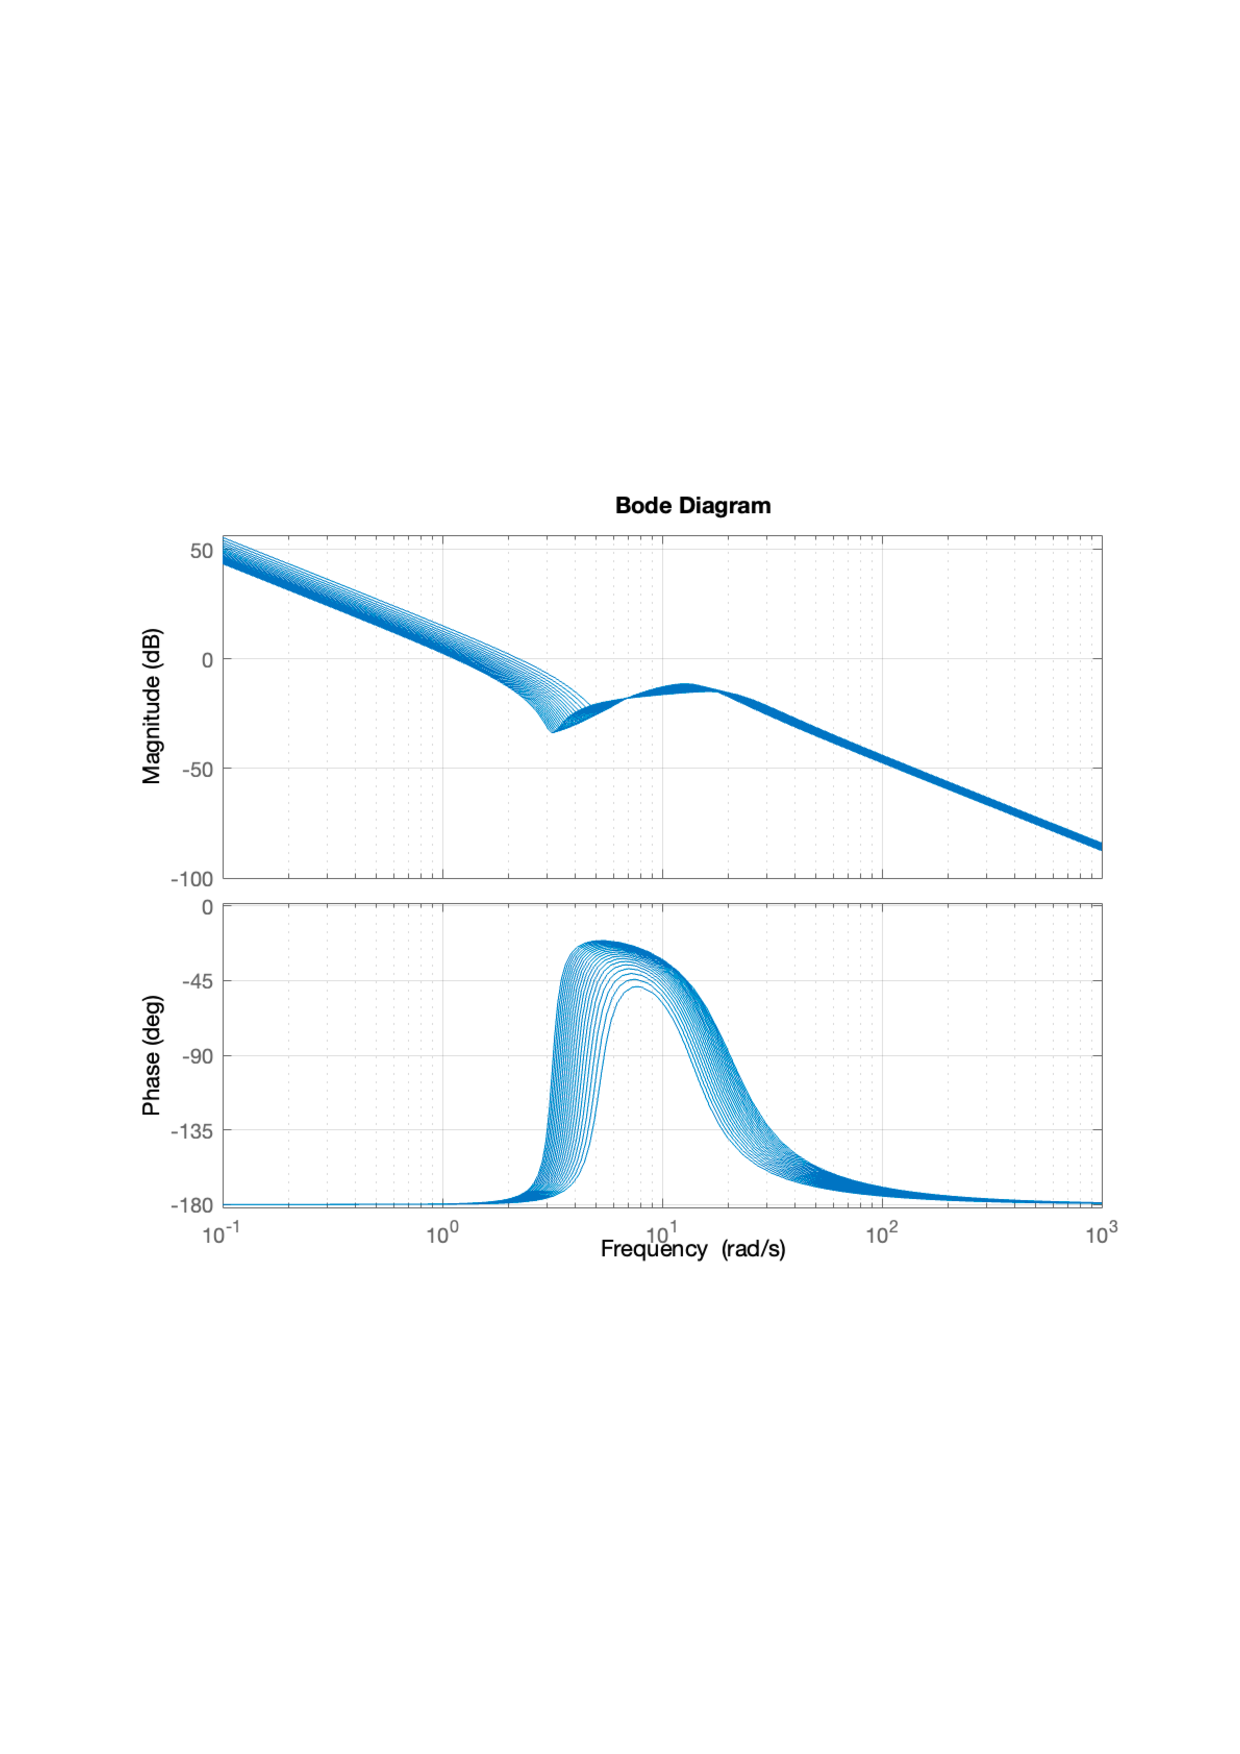
\includegraphics[width=\textwidth]
        {Figures/fig06a.pdf}
            \caption{$P_c\ uncertain$}
        \label{fig:fig06a}
    \end{subfigure}
    \begin{subfigure}[b]{0.45\textwidth}
        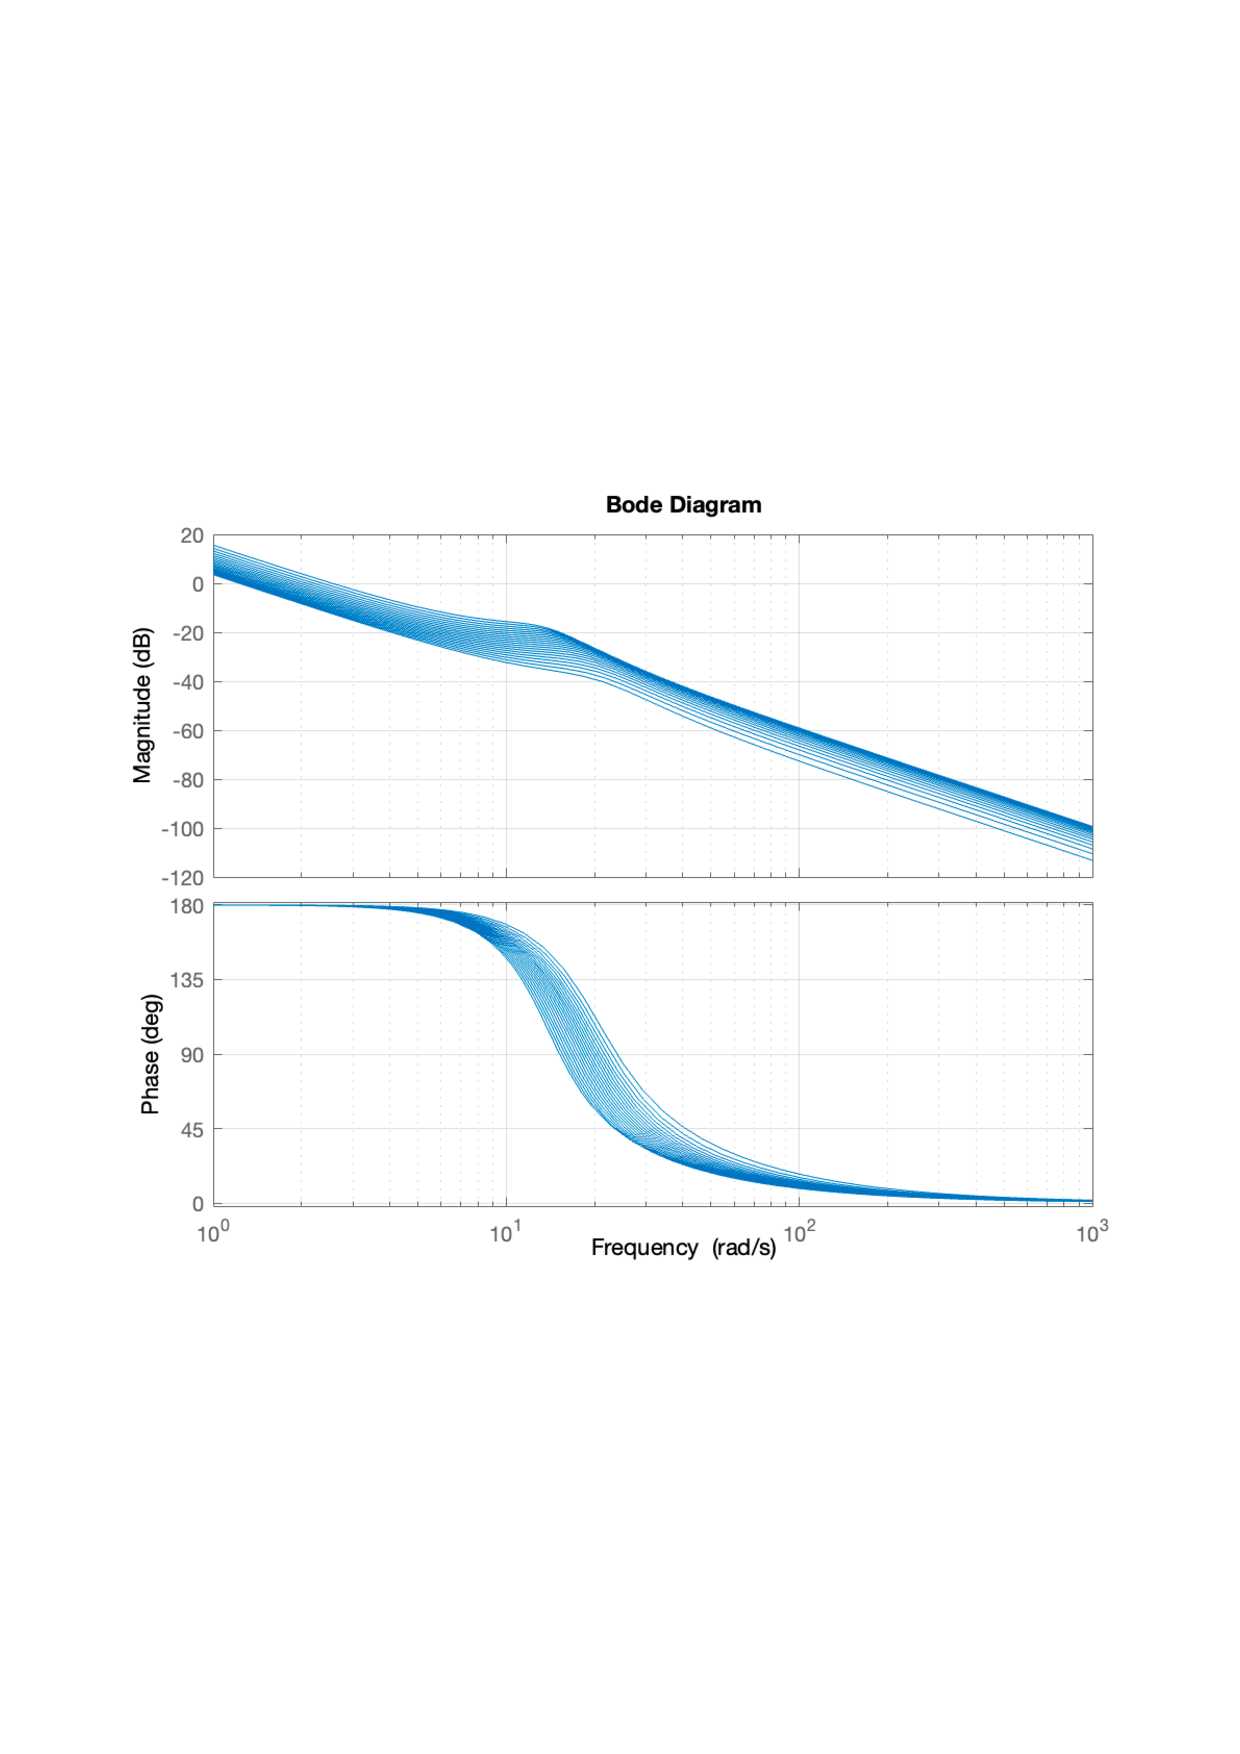
\includegraphics[width=\textwidth]
         {Figures/fig06b.pdf}
        \caption{$P_t\ uncertain$}
        \label{fig:fig06b}
    \end{subfigure}
    \caption{Bode Graphs for the uncertain Plants}
    \label{fig:fig06}
\end{figure}
\\\\Once we close the loop, we use $robstab(...)$ to check the stability margins and the "destabilizing" values for the parameters.\\\\
For the minimum phase plant, we find that all stability margins are greater than one (meaning the \textbf{controller is robustly stabilizing the system inside our ranges of parameters}). This holds true also for the non minimum phase plant, but only with the controller designed with the "compromise" paradigm.
\\\\ 
As for the "greedy" controller, the situation is different. In fact there are values of the parameters inside the chosen range that make the closed loop system unstable and therefore such controller is not robust with respect to the parametric uncertainties introduced above. 
\\\\ As a matter of fact choosing $J_{unc} = 0.2313,\ \Phi_{unc}'(0) = 7.8177,\ \Phi_{unc}(L)= -2.6881,\\ \omega_{unc} = 15.2361,\ \omega_{unc}^2=232.9874,\ \zeta_{unc} = 0.3624$ we have that the Nyquist plot for the Loop function passes through the point (-1,0) (Fig.~\ref{fig:fig07}) and therefore the controlled plant has purely imaginary poles. For the same reason, the sensitivity functions will present an infinite peak and it won't be possible to track any constant reference: the presence of purely imaginary poles translates into oscillations even at steady state.

\begin{figure}[h!]
    \FigureSeven
    \caption{Nyquist Plot for "Greedy controller" in critical case}
    \label{fig:fig07}
\end{figure}

\subsection{Unstrured Full Complex Uncertainty}
Let's now "exaggerate" our requirements by using an unstructured full complex uncertainty representation. This choice is much more conservative and actually not necessary at this point, but it's a good indicator of "how robust" our controllers actually are.
\\\\
The basic idea is to use an unstructured $\Delta(s)$ which is represented as the unit disc and approximate the "real" uncertainty to a disc in the complex plane. Then, using the command $ucover()$, we find a frequency-dependent radius ($w_a(s)$ or $w_m(s)$ as for the chosen representation) that describes the "level of uncertainty" at each frequency.
\subsubsection{Unstructured Additive Uncertainty}
Using the full complex additive formulation: $P = P_{nom} + w_a \Delta$, we get that the controllers found are \textbf{not robust with respect to this kind of modeling for the uncertainties}.
\\
One way to visualize it is using the Nyquist plot of the loop function. We know that the uncertainty can be visualized as a circle of radius $|C(j\omega)w_a(j\omega)|,\ \forall \omega$. For robust stability, none of those circles must encircle the critical point (-1,0) of the complex plane. 
\\Fig.~\ref{fig:fig08} shows the plot relative to the uncertain base loop function (the one for the tip would be very similar). For better visualization, we rescaled all the radia by the $"UpperBound"$ value and we plotted in green the circle relative to the $"CriticalFrequency"$ (both values provided by $robstab(...)$. Thanks to the scaling, the uncertainty circle boundary relative to the critical frequency passes exactly through (-1,0).
\begin{figure}[h!]
    \FigureEight
    \caption{Nyquist Plot for Base Loop function with rescaled weights (circles)}
    \label{fig:fig08}
\end{figure}
\\It's no surprise that the necessary and sufficient condition for robustness is violated by both systems: $\|\mathbf{w}_a(s) C(s) S_{\text{nom}}(s)\|_\infty > 1$ (instead of < 1)
\subsubsection{Unstructured Multiplicative Uncertainty}
On the other hand, using a multiplicative modeling for the uncertainty appears to be a better choice (not too conservative). Using $ucover()$ to find the multiplicative weight $w_m(s)$  and the full complex multiplicative formulation ($P = P_{nom}(1 + w_m\Delta)$) we get that both controllers for the MP and NMP plants are robust.
As a matter of fact, they both satisfy the necessary and sufficient condition for robustness:
$\|\mathbf{w}_m(s) T_{\text{nom}}(s)\|_\infty < 1$
\subsection*{Remark: Full Complex Robust Stability}
We might be curious to investigate why the additive representation gives opposite results with respect to the multiplicative one.
\\One of the possible reasons is indubitably the choice of the two weights $w_a(s),\ w_m(s)$. Fig.~\ref{fig:fig09} shows how the additive weight (in this case for the "base plant") is significantly more conservative than the multiplicative one.
\begin{figure}[h!]
    \FigureNine
    \caption{Weights comparison: additive vs multiplicative}
    \label{fig:fig09}
\end{figure}
\\Therefore, not only the full complex representation is by itself much more conservative for our real parametric uncertainty, but the choice of the weights can further accentuate the situation and lead to misleading results.
\subsection{Unmodeled Dynamics}
Considering the fact that we're approximating an infinite-dimensional, non-linear system with a linear and finite-dimensional one, it's reasonable to add some uncertainty deriving from the unmodeled dynamics. In particular, we model higher uncertainty at high frequency and small to none at low frequency.
\\ \\
To do so, we use the classic weight:
\begin{equation*}
    w_u(s) = \frac{r_0 (1 + \tau/r_0 s)}{(1 + \tau/r_\infty s)}
\end{equation*}
\begin{figure*}[h!]
        \centering
        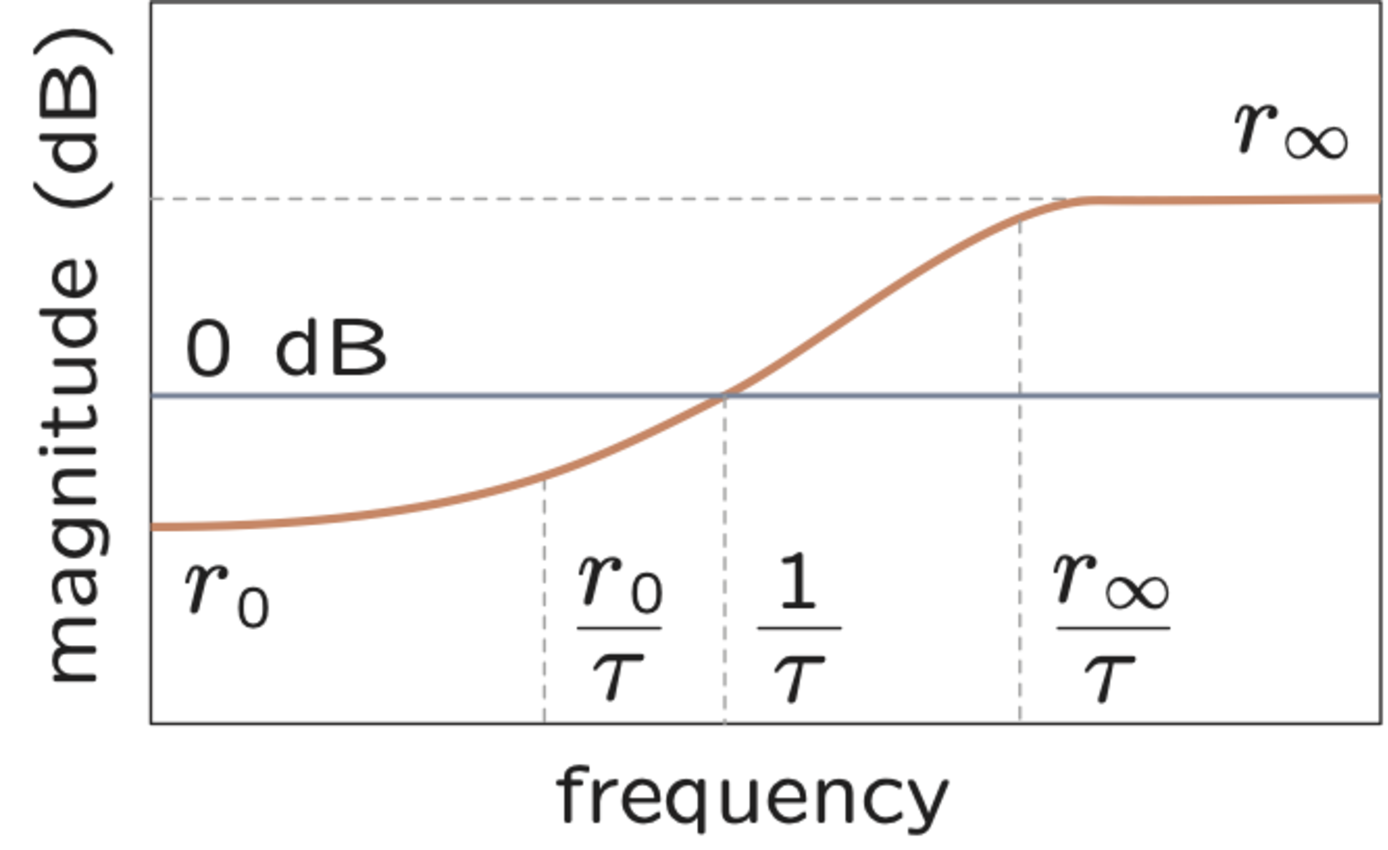
\includegraphics[width=0.4\textwidth]{Figures/unmodelled.pdf}
\end{figure*}
\\In particular, we impose a 1\% uncertainty at low frequency up to 200\% at high frequency, passing through 100\% at $\omega = 25$, while keeping all parametric uncertainties previously defined.
\\\\We consider once again the "base plant" and adopt a multiplicative representation. The uncertain plant is modeled as: 
\begin{equation*}
    P_{U}(s) = P_{nom}(s)(1+w_{U}(s) \Delta_{U}(s)), \ \ \|\Delta_{U}(s)\|_\infty \le 1
\end{equation*}
Where $w_{U}(s) \Delta_{U}(s)$ contains both parametric uncertainty and unmodeled dynamics.
\begin{figure}[h!]
    \FigureTen
    \caption{Nyquist loop Function for parametric uncertainty and unmodeled dynamics}
    \label{fig:fig10}
\end{figure}

From the Nyquist plot in Fig.~\ref{fig:fig10} we notice that the controlled system is robustly stable. 
To double check, we can observe also that $ucover(...)$ gives stability margins greater than one and the $H_\infty$ condition is satisfied $\|\mathbf{w}_m(s) T_{\text{nom}}(s)\|_\infty < 1$


\subsection{Neglected Dynamics}
Let's look at the uncertain plant Bode magnitude plot in Fig.~\ref{fig:fig06a}. We notice that, after a certain frequency, the dynamics can be approximated to a double integrator of the kind $P_n = \frac{K_n}{s^2}$.\\
\\ At this point, we use the $zpk(Pc_unc)$ command to find the nominal "gain" in the zero-pole-gain representation and choose it as our $K_n$. We can therefore rewrite the uncertain base plant as $Pc_{unc} = P_n * P_{neglected}$, with the second term being the residual dynamics (containing all the uncertainties).
\\\\
We then adopt the multiplicative formulation and rewrite everything as $P_{tot} = P_n(1+w_{neg}\Delta)$, with $w_{neg}$ a proper weight that "covers" the uncertainty from the neglected dynamics and the parametric uncertainty.
\\\\
We can now design an $H_\infty$ nominal controller for the $P_n$ plant, meaning the gain-double-integrator simplified dynamics. We choose "lousier" specifications knowing that a large uncertainty is now present w.r.t. the original uncertain plant.
\\\\
At this point, we verify that the controller found \textbf{robustly stabilizes the uncertain plant}, even after neglecting all the uncertainties AND a large part of the dynamics.
\begin{figure}[h!]
    \FigureEleven
    \caption{Nyquist loop Function for neglectd dynamics}
    \label{fig:fig11}
\end{figure}
\\
As per usual, we have that the stability margin's bounds are greater than one, the uncertain Loop Function Nyquist plot stays out of the critical point (Fig.~\ref{fig:fig11}) and $\|\mathbf{w}_m(s) T_{\text{nom}}(s)\|_\infty < 1$ (for numerical errors of Matlab, it's actually 1.012 but everything else checks out).
\\\\
As a final check, we also notice (not surprisingly) that using the same controller on the original uncertain plant (real structured parametric uncertainty), we still have robust stability.
\section{Extension: Augmented Plant Framework}
Let's now try to work with the augmented plant framework. Let's consider the $\theta_c$ as \textbf{measured variable} and the tip tracking error $e_{tip} = r - \theta_{tip}$ and the control effort $u$ as \textbf{performance variable}.
\\The resulting augmented plant, completed with the performance weights and shown in Fig.~\ref{fig:fig12} , can be written as:
\begin{equation}
\begin{bmatrix}
z_1 \\
z_2 \\
v
\end{bmatrix}
=
\begin{bmatrix}
w_S & -P_t w_S \\
0 & w_u \\
1 & -P_c
\end{bmatrix}
\begin{bmatrix}
w \\
u
\end{bmatrix}
\end{equation}
with: $z = [e_{tip}\ u]^T$;\quad$v = r - \theta_c$;\quad$w = r$

\begin{figure}[h!]
    \FigureTwelve
    \caption{Augmented Plant Block Diagram}
    \label{fig:fig12}
\end{figure}
We can use the augmented Plant $P_e$ to design an $H_\infty$ optimal controller, and then test it on the original (no weights) plant.
\\\\
Such design is made through the Matlab command $hinfsyn(\dots)$. However, for numerical Matlab computations beyond my understanding, we have two major issues:
\begin{enumerate}
    \item The only properly working algorithm for $hinfsyn(\dots)$ is the "LMI" for this system. Using the default Riccati solver, Matlab cannot find any stabilizing controllers or finds controllers with ridiculously low bandwidth.
    \item Even the "working" LMI solver finds solutions that are often counter-intuitive with respect to the weights' design. Moreover, most of the times imposing a $gamTry$ parameter (value of $\gamma > 1$ that we take as good) results in a better controller than the $H_\infty$ optimal one.
\end{enumerate}
For these two reasons, the weight choice was made mostly via trial and error. Despite that, we still found one interesting results (not very "transparent" in terms of weights).
\\\\
Any choice of the "regular" weights (as shown in Fig.~\ref{fig:fig12}) leads to a designed controller that is outperformed by the one designed by the $mixsyn(..)$ command (an example can be found in the Matlab file). However, if we remove all the weights and only scale $y_t$, for some reason the optimization algorithm works better and finds better performing controllers. 
Imposing $w_{yt} = 10; \gamma_{try} = 9.5$ (like I said, a bit counter-intuitive), $hinfsyn(\dots)$ finds a stabilizing controller that outperforms the one found with "classic" mixed sensitivity design.
Fig.~\ref{fig:fig13} shows an even faster convergence at the desired position, despite having an output feedback on a measured variable which is not the same as the one used for performance evaluation (base vs tip). Of course the price to pay is in terms of control effort, which is however still in a more than acceptable range.
\begin{figure}[h!]
    \begin{subfigure}[b]{0.45\textwidth}
        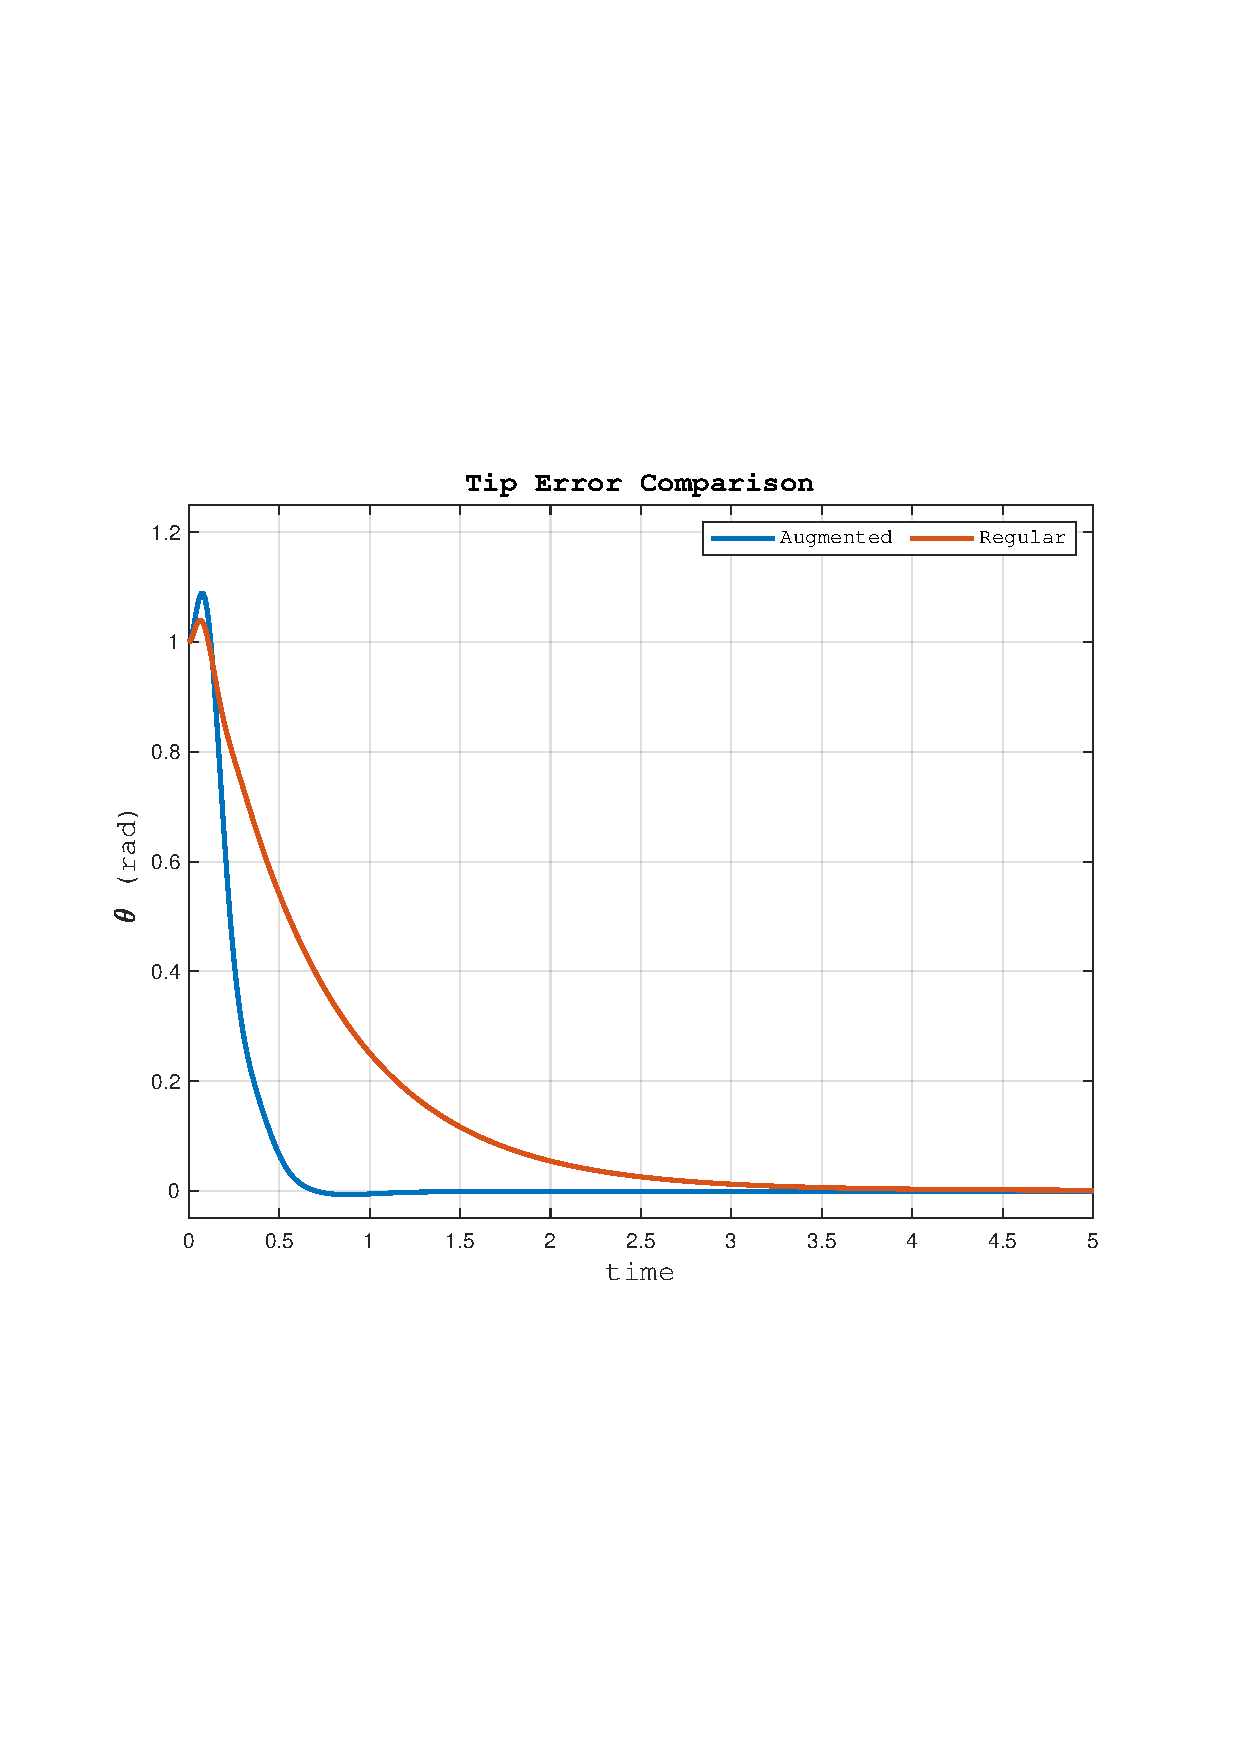
\includegraphics[width=\textwidth]
        {Figures/fig13a.pdf}
            \caption{Error convergence comparison}
        \label{fig:fig13a}
    \end{subfigure}
    \begin{subfigure}[b]{0.45\textwidth}
        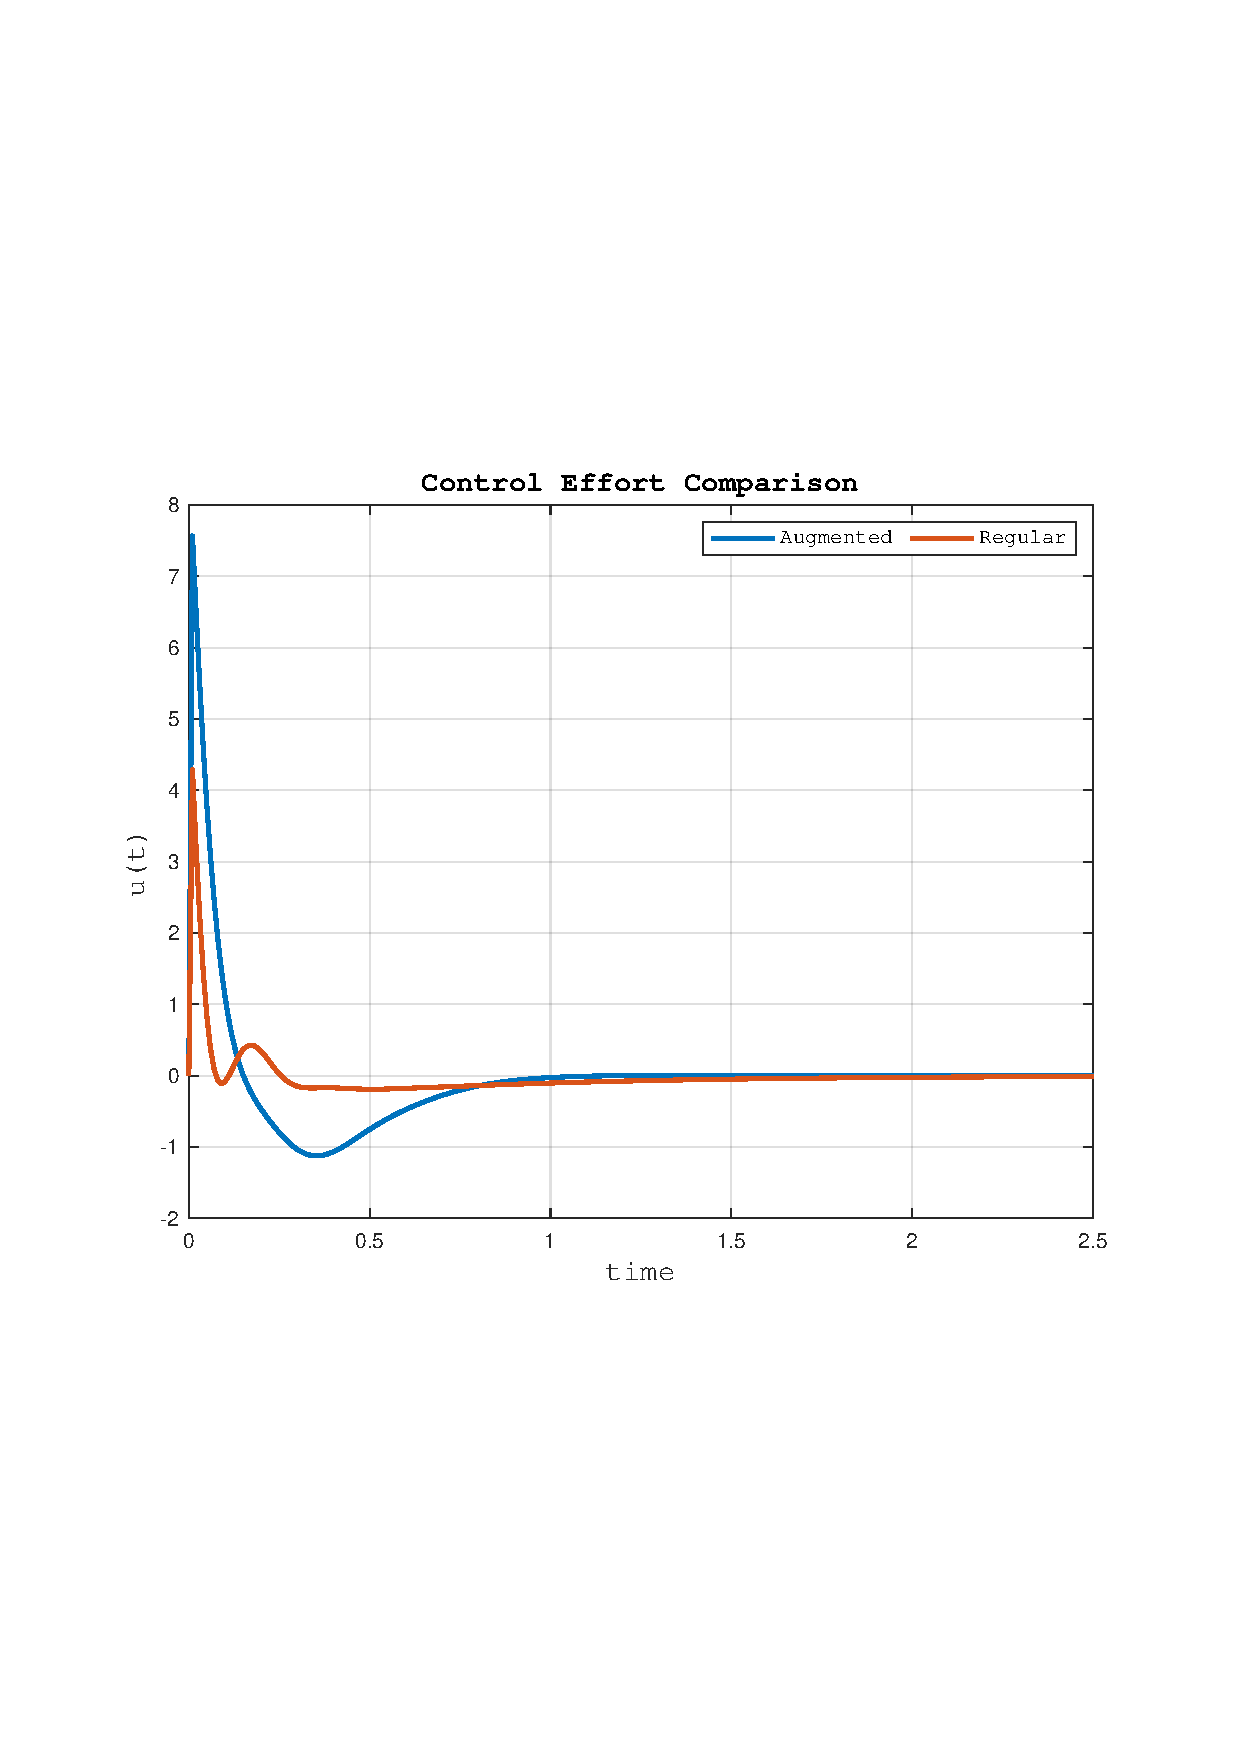
\includegraphics[width=\textwidth]
         {Figures/fig13b.pdf}
        \caption{Control effort comparison}
        \label{fig:fig13b}
    \end{subfigure}
    \caption{Performance comparison for $H_\infty$ controllers designed with augmented plant vs regular mixsyn}
    \label{fig:fig13}
\end{figure}
\end{document}
